At the end of section~\ref{chp:SOLO_Quite_time}, \citet{Mason-2021-SolOQuietTime} reported the radial gradient of \ac{ACR} oxygen and helium-4 with energies of 4.4 MeV/nuc within 1 au. The analysis was based on the measurements from the \ac{SIS} instrument in 2020, and particle intensities were plotted as a function of three radial locations. Due to limited counting numbers, the flux uncertainties of flux were relatively large. However, the results still indicate a positive and small gradient for oxygen compared to the observations from Helios and \ac{PSP} \citep{Rankin2021ApJ,Marquardt2018AA}.

As of 2023, the changing solar activities and the solar modulations have also influenced \acp{ACR} in the inner heliosphere as they propagate inward and diffuse throughout the heliosphere. Those changes are reflected in the variation of \ac{ACR} intensities and potentially in that of the radial gradient.
Meanwhile, the \ac{SolO} has completed its fifth orbit and continues its journey in the inner heliosphere. The \ac{HET} on board the \ac{SolO} has been measuring helium of tens of MeV/nuc during the last two years witnessed the change of solar activities and solar modulations.

Therefore, in this chapter, we investigate new \acp{ACR} observations in the inner heliosphere and in the new solar cycle, utilizing new data from the \ac{HET} on board \ac{SolO}. We present the spectra and radial gradient of \ac{ACR} helium in the inner heliosphere between 2020 and 2022, taking into account possible interuptions such \acp{SEP}, periodically occurring \ac{CIR} and long-term solar modulation. Moreover, we use helium flux measurements from the \ac{EPHIN} on board \ac{SOHO} to derive the flux ratio between \ac{SolO} and \ac{SOHO}/\ac{EPHIN}. By so, we remove the effect of solar modulation. Preliminary results indicate consistency between \ac{HET} and \ac{EPHIN}, and the radial gradient of helium-4 aligns closely with previous results from \ac{PSP}, considering the uncertainties. The variation of the helium radial gradient is also discussed in the early phase of solar cycle 25

The details of the data analysis and results are given below. Noting that results are still in the preliminary phase. We will continue analyzing the data and preparing the final publication, which will be submited to Astronomy and Astrophysics in the near future.


\section{Background}

The \ac{ACR} are the energetic ionized neutrals that are widespread in the heliosphere and are predominant in the energy range of tens of MeV/nuc. The source of \ac{ACR} is believed to be the blunt temination shock located at the boundary of heliosphere \citep{McComas2006GeoRL}. Since the \ac{ACR} was first discovery in 1970, scientists have confirmed the observations of \ac{ACR} helium, oxygen, neon, and also protons in the outer heliosphere. \citep{Garcia1973ICRC,Hoverstadt1973PhRvL,McDonald1974ApJ,Potgieter2013LRSP}

Generally, the transport of the cosmic rays in the heliosphere are described by the interaction between charged particles and the solar wind as well as its embedding large scale solar magnetic field. The different physical processes that affection the propagation of particles are (a) diffusion caused by the irregular magnetic field, (b) adabitic energy loss and convection due to the expanding solar wind, and (c) gradient and curature drift leaded by the heliospheric magnetic field
Though the cosmic ray transport equation have generally described and modeled those basic processes \citep{Parker1965Pss,Jokipii1977ApJ,Jokipii1981ApJ,McDonald2001ICRC}, the detailed roles of each components in the inner heliosphere and how the new measurement affected by the varying solar magnetic field are still not fully understood. \citep{Rankin2021ApJ}

In particular, spatial gradients provide valuable insights into the variation of drift effect of charged particle through consecutive solar cycle. As elucidated by \citet{Jokipii1977ApJ, Jokipii1979ApJ, Potgieter2013LRSP}, the drift direction of energetic particles differs during opposite solar polarities, which alternate approximately every 11 years, resulting in the form of a 22-year variation. Considering the recent solar activity minimum (\ac{SC} 24/25 in 2020) as an example, the solar magnetic field exhibits positive polarity. Consequencely, the positively charged ions drift inward from the south and north pole regions, while moving outward along the equatorial plane through the current sheet. Conversely, during the opposite polarity, ions drift inward from the equator and exit through the poles. Noting that the drift direction of electrons is opposite to that of ions. The drift effects are manifested in spatial gradients. Previous observtions from Voyager and Pioneer missions have indicated that the latitudinal gradient changes sign between two consecutive solar cycles belonging to different polarities, in agreement with predictions from tranport models \citep{Mckibben1979ApJ, Cummings1987GeoRL, Christon1986JGR}. Moreover, the magnitude of the radial gradient varies between between different polarity solar cycles \citep{Rankin2021ApJ,Rankin2022ApJ,Giacalone2022SSRv,Webber1981JGR,Marsden1999AdSpR}

%Despite of this, the precious radial gradient of the current solar cycle especially during the ininial phase of the new solar cycle are not measured and determined.
Acoording to \citet{Rankin2021ApJ}, the radial gradient of cosmic rays could be express as:
\begin{equation}
    g_r = \frac{1}{f}\frac{\partial{f}}{\partial{r}} = \frac{\partial{\mathrm{ln} f}}{\partial{r}}
    \label{eq:radial_gradient}
\end{equation}
Where $g_r$ denotes the differential radial gradient component under the assumption that the latitude gradient is negligible. It represents the change of the differentila flux, $f$ with respect to radial distance $r$. The radial gradient can be obtained by fitting the data to a linear equation using the least square method.


Benefiting from its unique orbit, with a cloest perihelion distance of 0.28 au, \ac{SolO}, launched on 2020, provides valuabel insights into the transport effects of the cosmic rays in the inner heliosphere by measuring the radial gradient of those particles.
In Fig.~\ref{fig:SOLO_orbit_info}, we present the orbit information of \ac{SolO} from Feb 2020 to May 2023. The top three panels display the radial distance to the Sun, Carrington longtitude and Carrrigton latitude of \ac{SolO}. As depicted in the top panel, \ac{SolO} has completed five orbits and is moving away from the Sun after passing its sixth perihelion. The closest distance to the Sun was achived during the fifth oribt in September of 2022. 
The carrington longititude of \ac{SolO} indicates its movement relative to a fixed longitude line on the Sun. Originally defined from the Earth's perspective, with a mean synodic period of approximately 27.2753 days, the Carrington system and its origin point are adapted to the \ac{SolO} coordinate system. 
Due to the greatly varying radius of the orbit, orbital periods of \ac{SolO} carrington rotations range between 26.6 and 35.8 days, slight differing from the period of the Earth. At the moment, the latitude of \ac{SolO} is constrained within a range of $\sim$ $\pm$8 degrees.
Additionally, we provide the radial distance and the longitudinal seperation between \ac{SolO} and Earth to illustrate the relative positions.

To better visualize and understand \ac{SolO}'s movement in the inner heliosphere and its relation to the Sun and Earth, we depict the orbit track of \ac{SolO} in two coordinate systems in Fig.~\ref{fig:SOLO_orbit_track}. The left panel shows the orbit in helioscentric ecliptic coordinate system, where the mean equinox are used as the reference direction of x axis. In this coordinate system, \ac{SolO}'s orbit exhibits an elliptical shape. Similarly, the right panel of Fig.~\ref{fig:SOLO_orbit_track} presetnt the orbit in a heliosgraphic coordinate system, with the Sun fixed in the the central and the Earth positioned at 1 au as blue dot. The x-axis is aligned the Sun - Earth direction. In this coordinate system, orbits appear twisted and undergoes changes in shape.

The color bars in both panels indicate the time sequence from February 2020 to May 2023. Carrington rotation numbers are marked at the beginning of each Carrington cycle and labeled next to the orbit track. The moving direction of spacecraft can been inferred from changes the numbers and colors.
%Obviously, when the spacecraft is located away the sun, the \ac{SolO} is moving in a limited region, with hardly changed longtitude in one carrington rotation. Conversely, the longitudinal changes are large when \ac{SolO} rapidly pass by the sun. Between them the radial distance change quickly. 


%In this report, we organized the content as following: We first introduce the data and instrument we used in this work, which including the SOLO/HET, SOHO/EPHIN, STEREO/LET and possiblely LND. In chapter 3 we give the overview of the observation of the helium-4 between 2020 and 2022 when in the second half, SEPs frequently happens and the overall cross-calibration between different instrument

%In section4, we explain the several kind of effect that could disturbe the constanct background and show how the result are affected by different method.  In the end, we conclude.



\begin{figure}
    \centering
    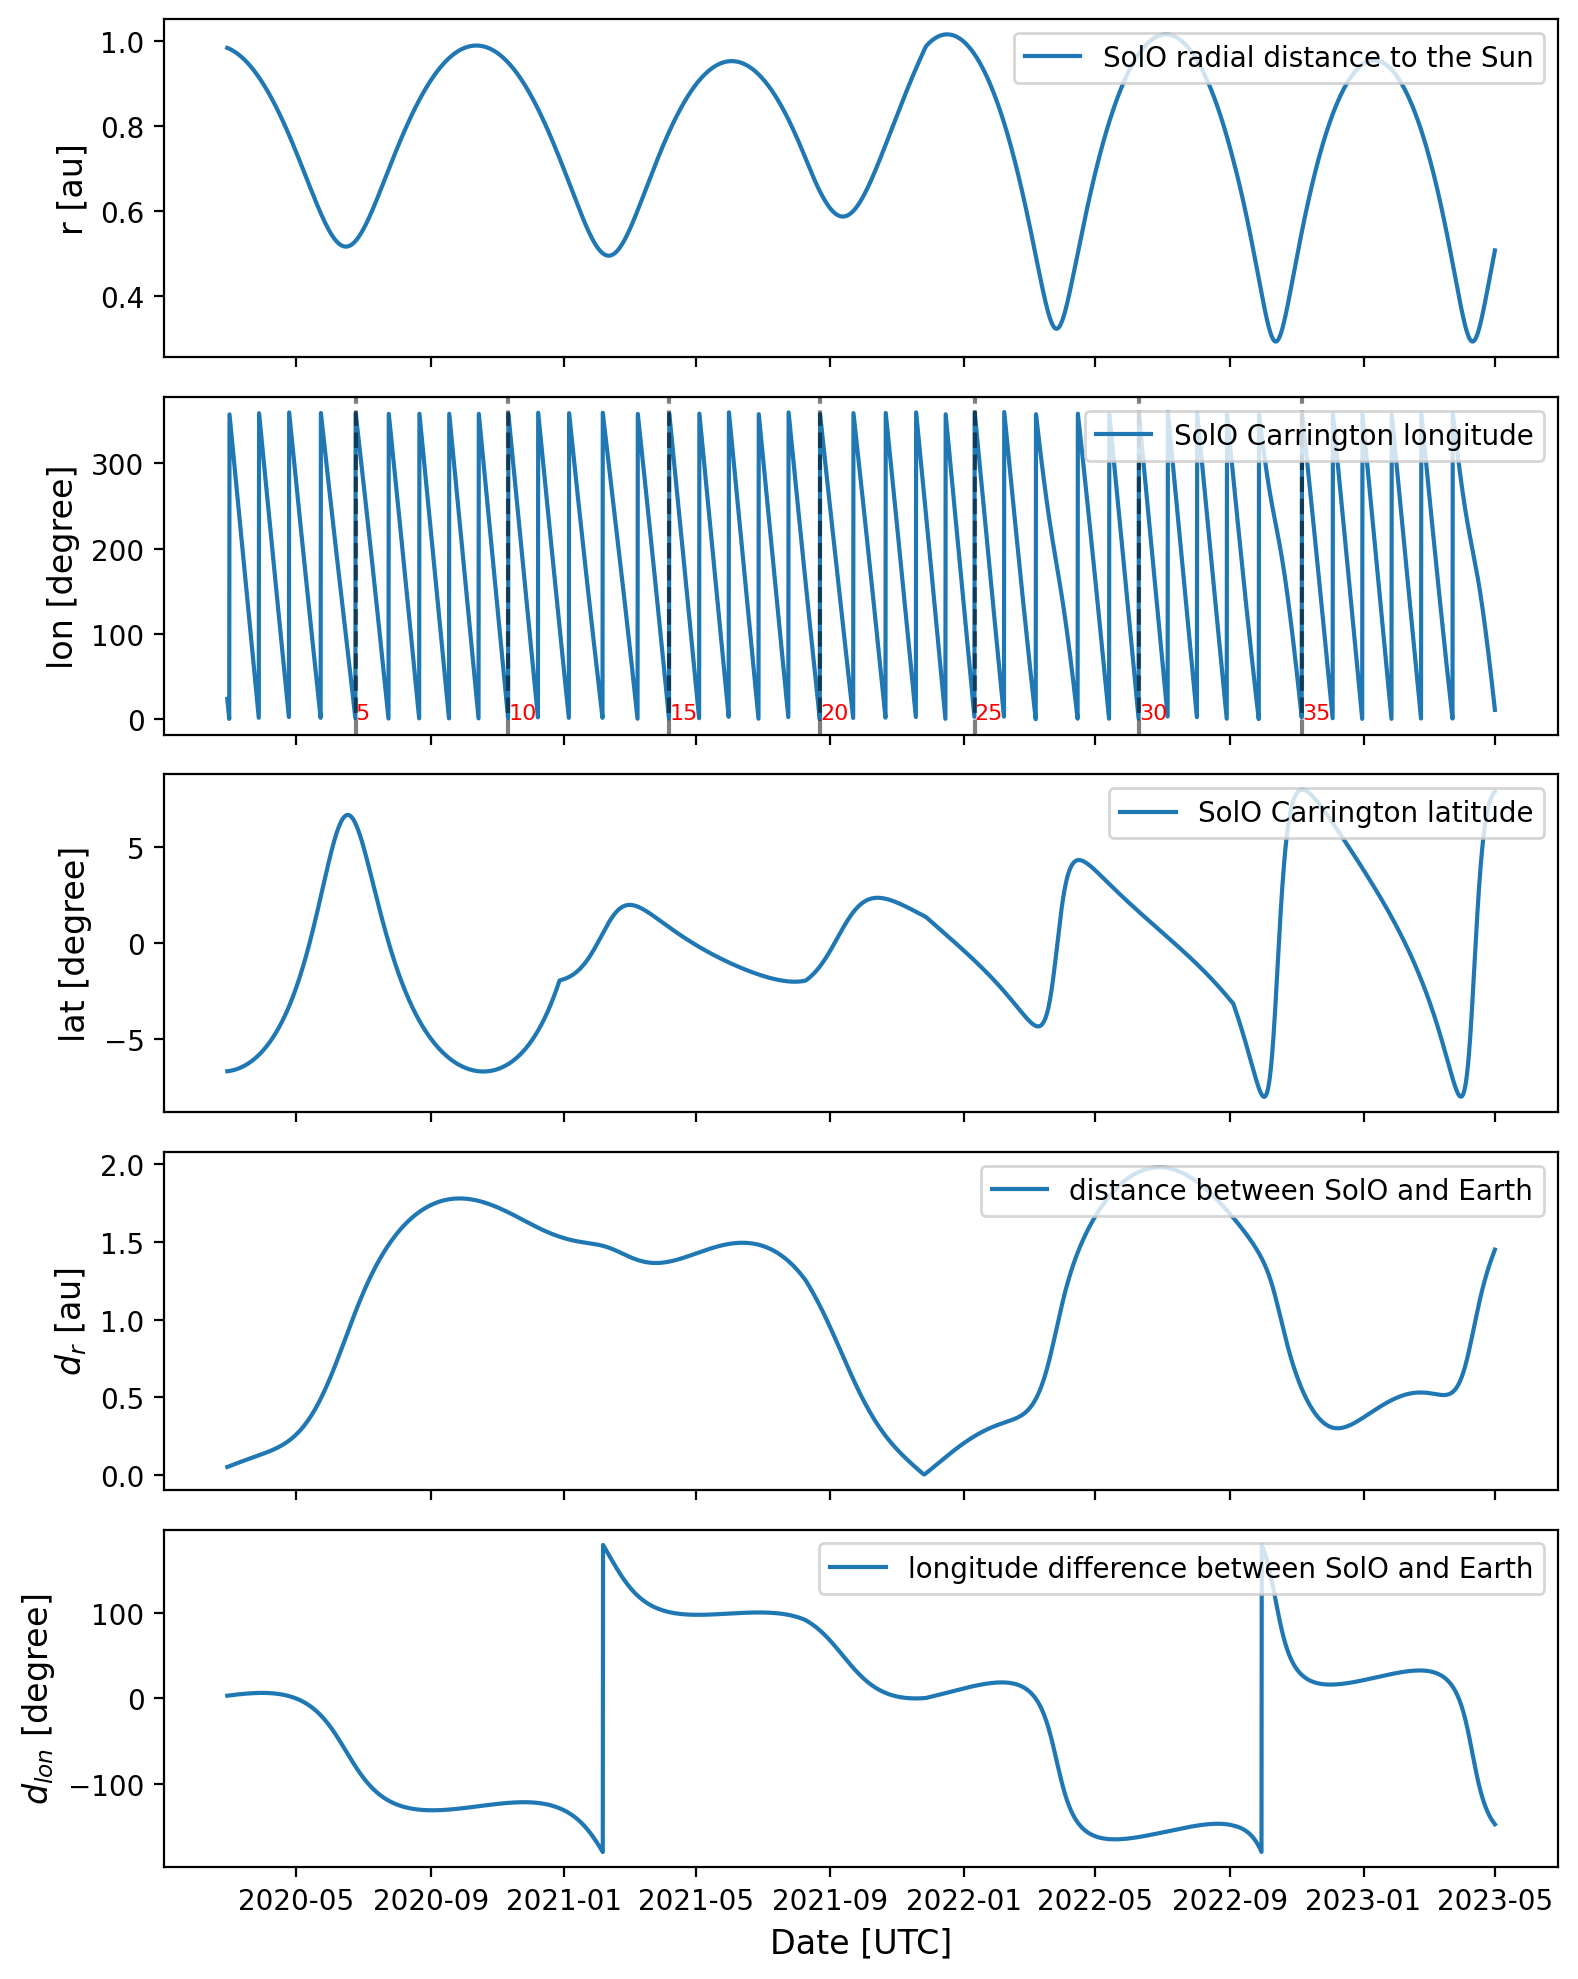
\includegraphics[width = 0.7\textwidth]{images/ACR/SOLO_orbit_helioscentric_3.png}
    \caption[The orbit variation of \ac{SolO} in carrington coordinate system]{(From top to the bottom) The variation of \ac{SolO}'s radial distance, Carrignton longitude, Carrington latitude as well as the distance and longitude seperation between \ac{SolO} and \ac{SOHO}. The time span covered in the figure ranges from February 2020 to May 2023. }
    \label{fig:SOLO_orbit_info}
\end{figure}
\begin{figure}
    \centering
    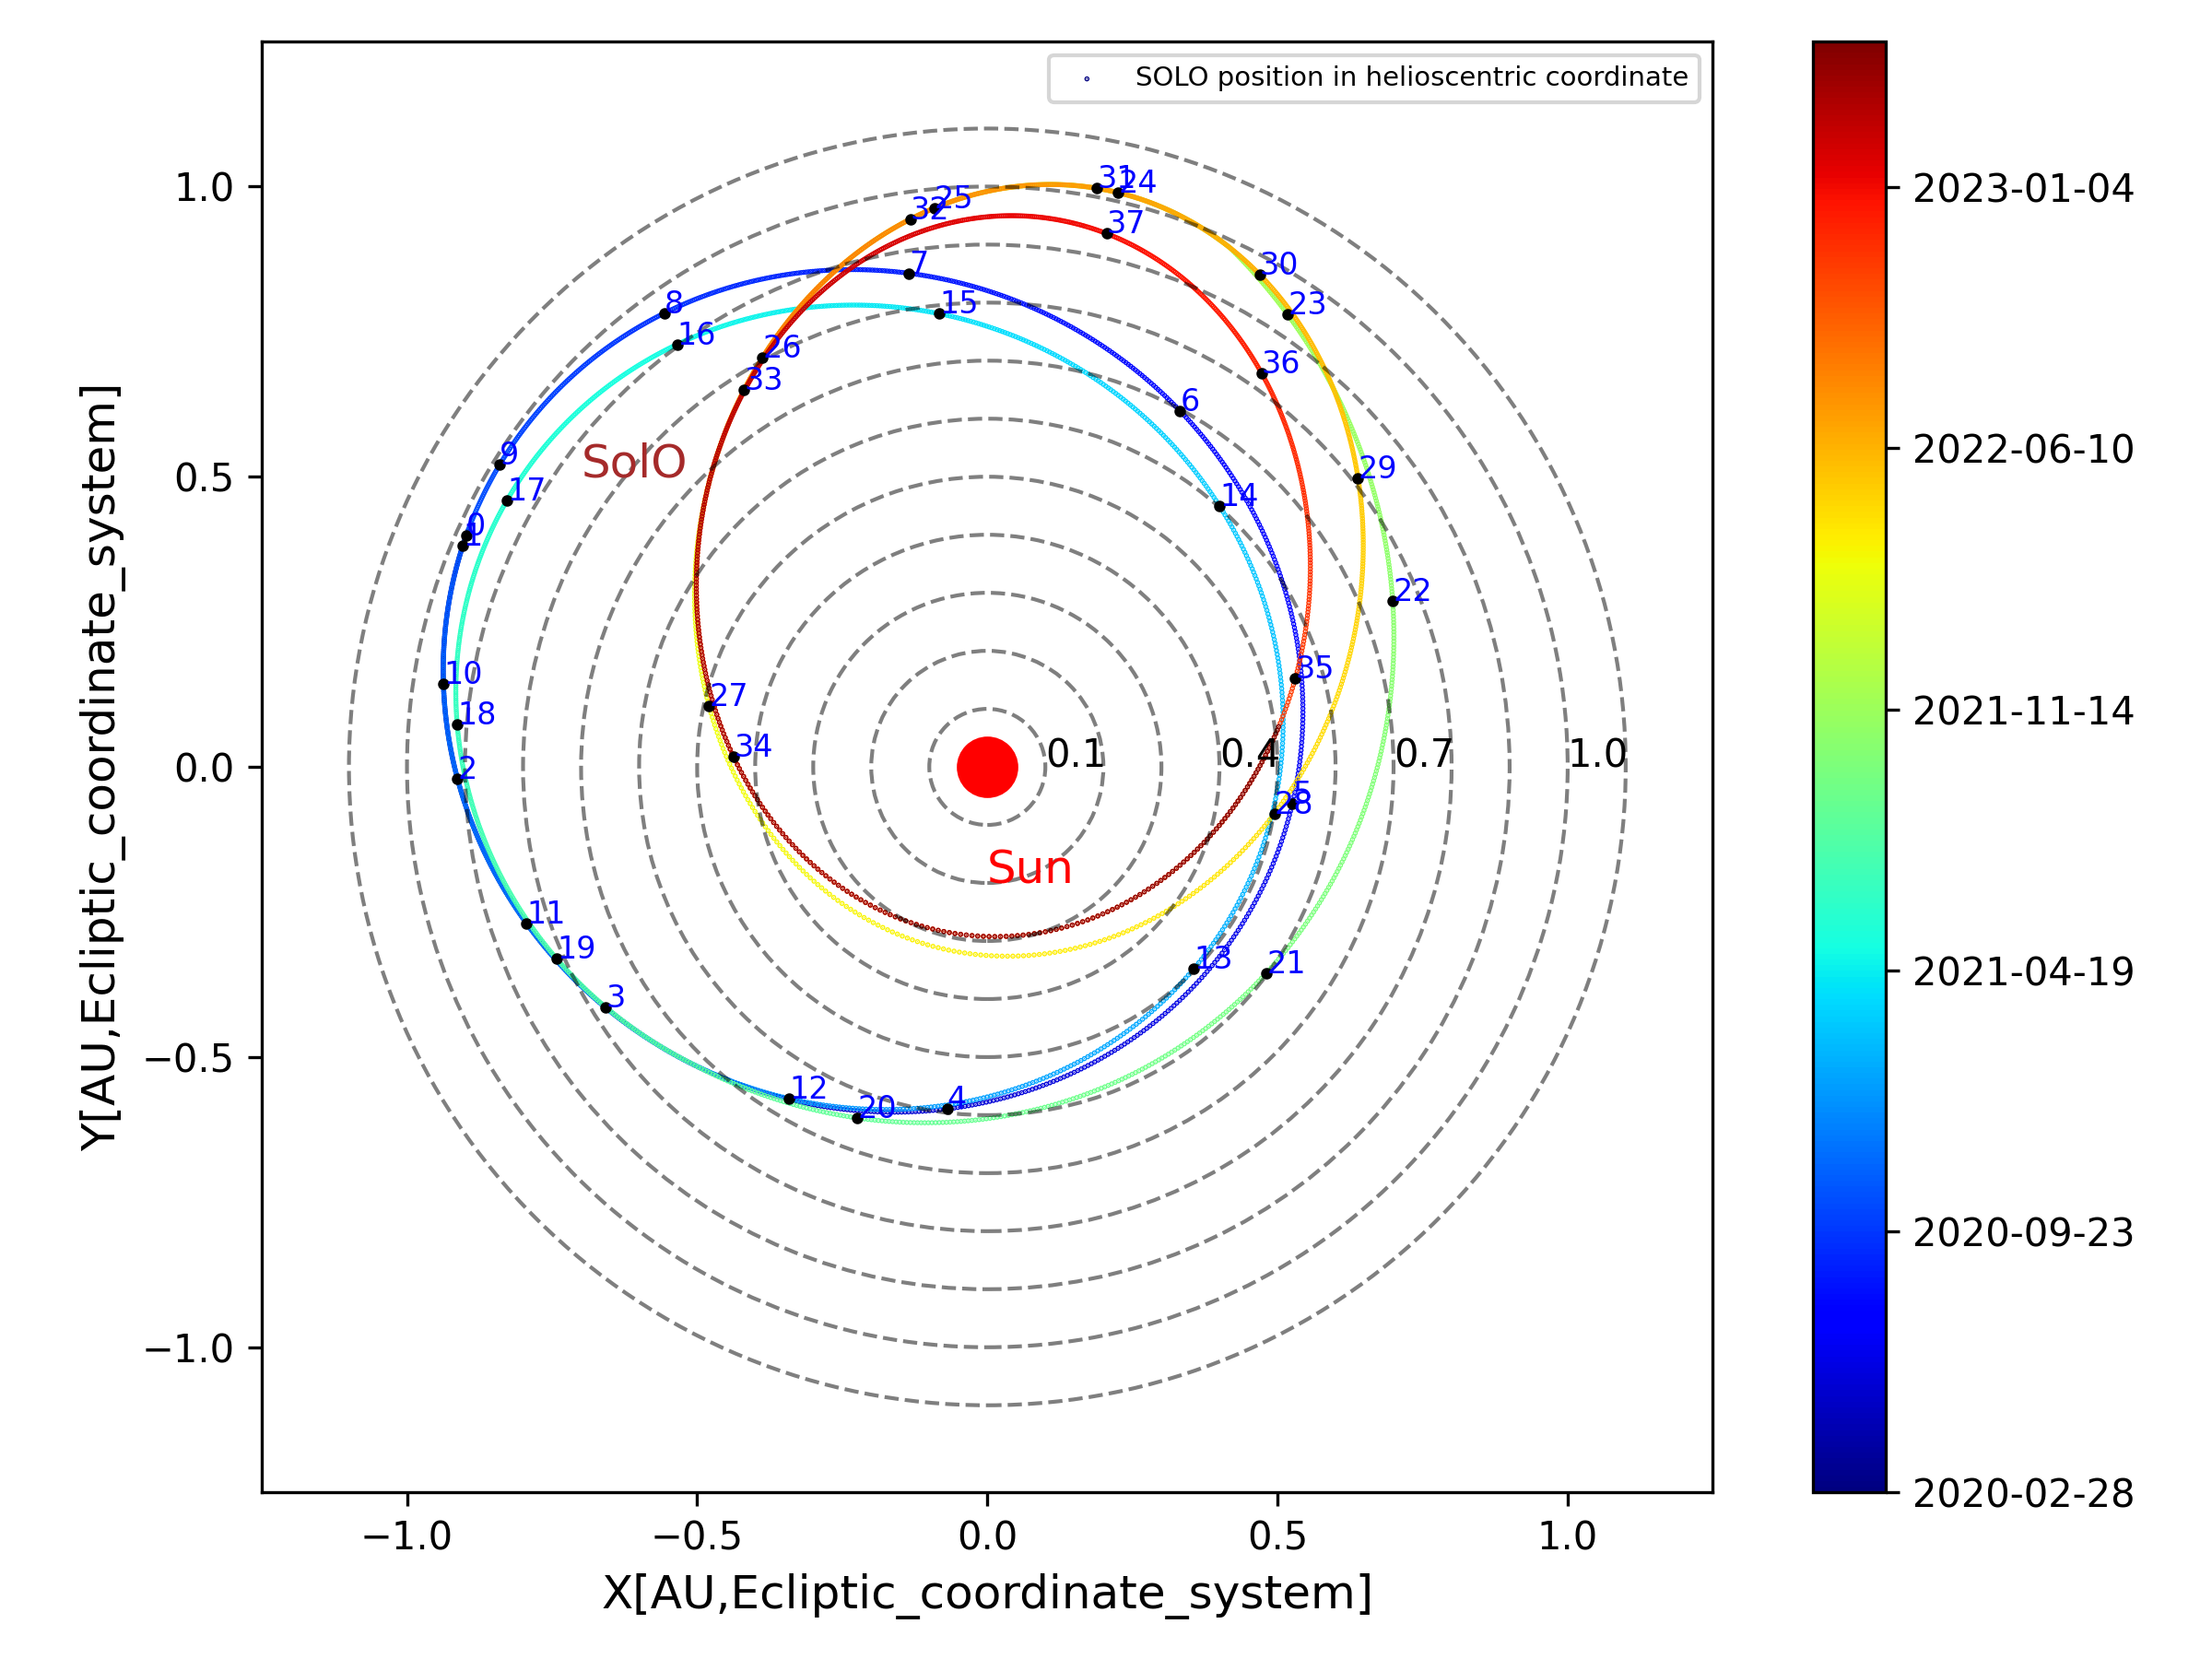
\includegraphics[width=0.45\textwidth]{images/ACR/SOLO_orbit_track_helioscentric_3.png}
    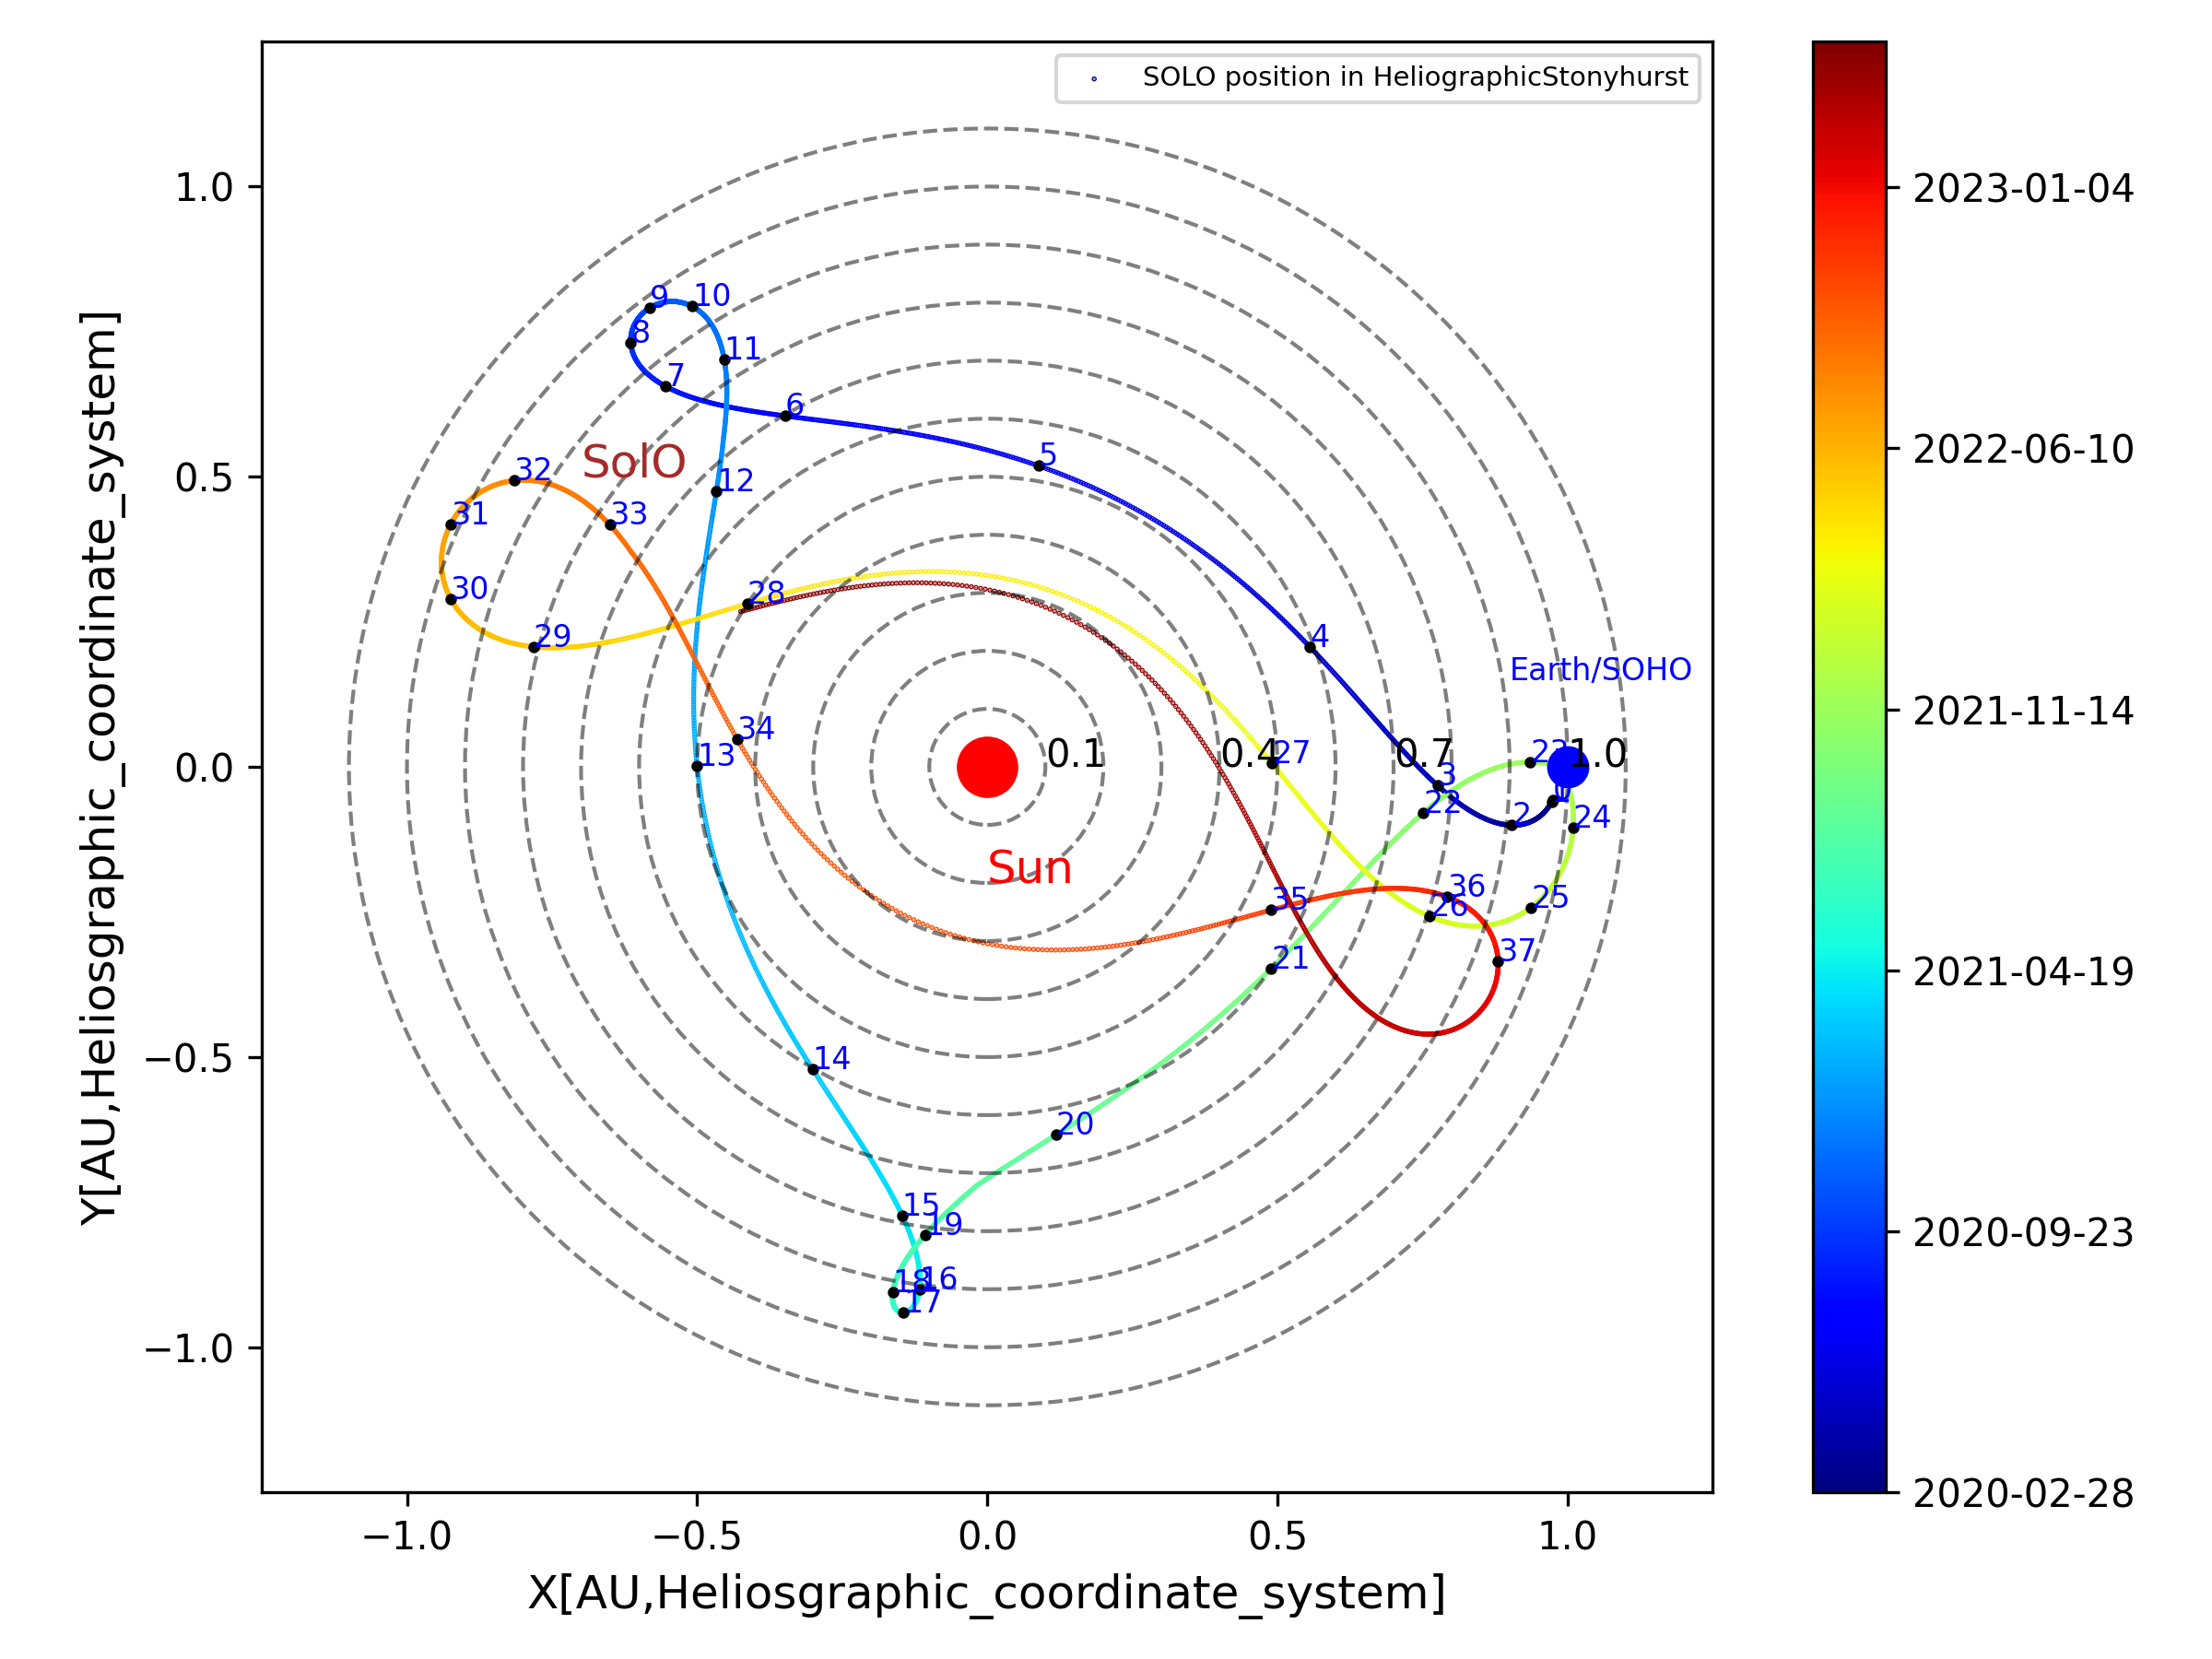
\includegraphics[width = 0.45\textwidth]{images/ACR/SOLO_orbit_stonyhurst_3.png}
    \caption[Orbit track of \ac{Solo}]{Left: The orbit track of \ac{SolO} in the helioscentric mean ecliptic coordinate system where the origin is the center of the sun, and reference line of x-axis points to the mean equinox and xy-plane is the ecliptic plane. Right: The orbit track of \ac{SolO} in the stonyhurst coordinate system. The Earth is fixed at 1 au is marked as the blue circle. 
    The numbers next to the track are Carrington rotation periods. The time span ranges from February 2020 to May 2023}
    \label{fig:SOLO_orbit_track}
\end{figure}




\section{Instrument}


The charged particles reported in this study are mainly from \acl{HET} onboard \ac{SolO} which measures ions in the energy range from tens of MeV/nuc to hundred MeV/nuc. Specifically, our focus lies on helium particles within the energy range of 10 MeV/nuc to 50 MeV/nuc, where the predominant particles are \acp{ACR} during the quiet time. Further details regarding the \ac{HET} measurement principle can be found in section \ref{sec:Solar_Orbiter} and \citet{RodriguezPacheco-2019-EPD}.

Similar to the analysis by \citet{Mason-2021-SolOQuietTime} for the \ac{SIS}, our analysis of the helium radial gradients measured \ac{HET} is also constrained by their counting statistics due to limited \ac{HET} geometry factors and lower helium intensities. To increase the count rate and reduce uncertainties, we employ two measures. First, we calculate a summation of the data collected from different instrument directions. \ac{HET} has four apertures pointing to sunward, anti-sunward, southward, and northward directions. Assuming the isotropic distribution of \acp{ACR}, the summation of particles from different directions reduces the uncertainties by half. Furthermore, we extend the energy bins of the \ac{HET} nominal data product and reconstruct the energy channels for particle stopping in detector C, covering the energy range of 10 - 20 MeV/nuc, 20 - 30 Mev/nuc, 30 - 40 Mev/nuc, 40 - 50 Mev/nuc. The specific boundaries of those bins are determined based on energy channels' values of nominal data products.

In addition to nominal data products designed to provide scientific measurements with high energy resolution and precious intensity, we utilize housekeeping data known as any(a1, b1) to identify the \ac{SEP} periods. Here \textit{a1} and \textit{b1} represent the front two sensors of \ac{HET} in the sunward unit. This level-2 trigger counts all particles with energy above the threshold of detector A or detector B, which is set to 50 keV in the nominal mode \citep{Elftmann-2020-PhD}, hence has more significant counting statistics. This trigger can detect energetic electrons, protons, and heavy ions without any element resolution, making it an ideal indicator of solar activities and \ac{SEP} events. 
%The periods are determined by the 3-sigma method \citep{Xu2017ApJ,Xu2020ApJ, Huttunen2005AA}, which is commonly used in determining the onset time of the \ac{SEP} event. In this method, if intensities of data points are about 3 time of standard devitaion higher than the background intensity, these data points are defined as the \ac{SEP}.


Apart from the measurement from \ac{SolO}, we also utilized the observations from \ac{SOHO}/\ac{EPHIN}, the \ac{ACESIS}, and the \ac{CRIS} onboard the \ac{ACE} and the \ac{LND}, for comparison purposes.  When considering the long-term variations in cosmic rays,  we take measurements from \ac{ACE}/\ac{ACESIS} as the baseline.


\section{Overview observation between 2020 and 2022 and the cross calibration between four instruments}

\subsubsection*{Spectra comparison between \ac{HET} and other instruments}
%\addtocontents{toc}{\protect\setcounter{tocdepth}{1}}
%%%%%% review to here.
Before deriving radial gradients of helium, let us quickly go through the \ac{HET} observations of heavier ions, such as helium, carbon, nitrogen, and oxygen, as Fig.~\ref{fig:overview} shows. After removing the possible \ac{SEP} periods we define below, the averaged spectra between 2020 and 2022 are displayed. \ac{SEP} periods are determined below, and the completed list of periods we removed can be found in Appendix \ref{Appendix:SEPlist}.

The \ac{HET} measurements are marked as diamonds of different colors, with red for helium-4, blue for oxygen, orange for carbon, and green for nitrogen.
All the helium nominal scientific data products from \ac{HET} are presented, which include particle stopping in detector B ($<$ 10 Mev/nuc), in detector C (10 - 100 MeV/nuc) and penetrating particles ($>$ 100 MeV/nuc), despite that the penetrating helium will not be used in the later analysis of \ac{ACR} gradient.
The penetrating helium comprises two populations depending on their primary energy: the barely penetrating helium marked as empty red diamonds and the fully penetrating particle with energy above 200 MeV/nuc. 

%%% here  ----
It is worth noting the potential issue of these penetrating data products. The intensity measured by two channels around 100 MeV/nuc are higher than the nearby channels and current we have no idea of the reason, probably due to the dead layer in front of each detectors\citep{Wimmer2021AA}. It also possible that the energy channels have not been properly calibrated.

Besides, the geometry factors of fully penetrating particles channels, i.e. the last three channels, are divided by a factor of two, to account for those \acp{GCR} equally incident from opposite directions. The current version of geometry factors are obtained based on the 2$\pi$ simulation by assuming the \ac{SEP} are highly anisotropic and arrive the detector from only one direction. 

The \ac{ACE} measurements are plotted as circles including filled circles representing \ac{ACESIS} and empty one for \ac{CRIS}. Unfortunately, \ac{ACESIS} only measured helium with energy below 15 MeV/nuc.
The helium data from \ac{SOHO}/\ac{EPHIN} are shown as the purple squares and the \ac{LND} measured helium-4 are shown as the brown triangles. Their measurement cover the \ac{ACR} energy range between 10 - 50 MeV/nuc.

The cross-comparison of the averaged spectra of all particle species in Fig.~\ref{fig:overview} reveals a general agreement between different instruments despite their distinct positions. This agreement indicates the reliable measurement of the \ac{SolO} and also \ac{LND}, which we for the first time report the helium-4 spectrum. Futhermore, the flat helium spectra between 10 MeV - 50 MeV/nuc and the higher intensity of oxygen and nitrogen at 10 MeV/nuc clearly demonstrate the presence of the \ac{ACR} components in the inner heliosphere. 
Later in Fig.~\ref{fig:helium_spec_1au}, we specifically focus on the helium-4 spectra based on the measurement when \ac{SolO} was positioned between 0.95 and 1 au. The time periods we selected in the last two years are given in Tabel \ref{tab:1AU_period}, which consist of the start time, end time and the distance from \ac{SolO} to the Earth.
Similarly, the \ac{EPHIN} and \ac{HET} helium of energy above 10 MeV/nuc show  the consistency in averaged spectrum. However, the discrepancy appear on the energy channel below 10 Mev where the intensity of \ac{ACESIS} is about 2 time higher than \ac{EPHIN}. Besides, the \ac{LND} spectrum appears generally higher than the other measurements and it also has larger error bars. This due to the limited operation time on the lunar surface (see section \ref{sec:change_4_LND}). As a result, we utilize the \ac{EPHIN} and \ac{HET} helium measurement within the energy of 10 to 50 MeV/nuc in the susequent analysis.



\begin{figure}[!htb]
    \centering
    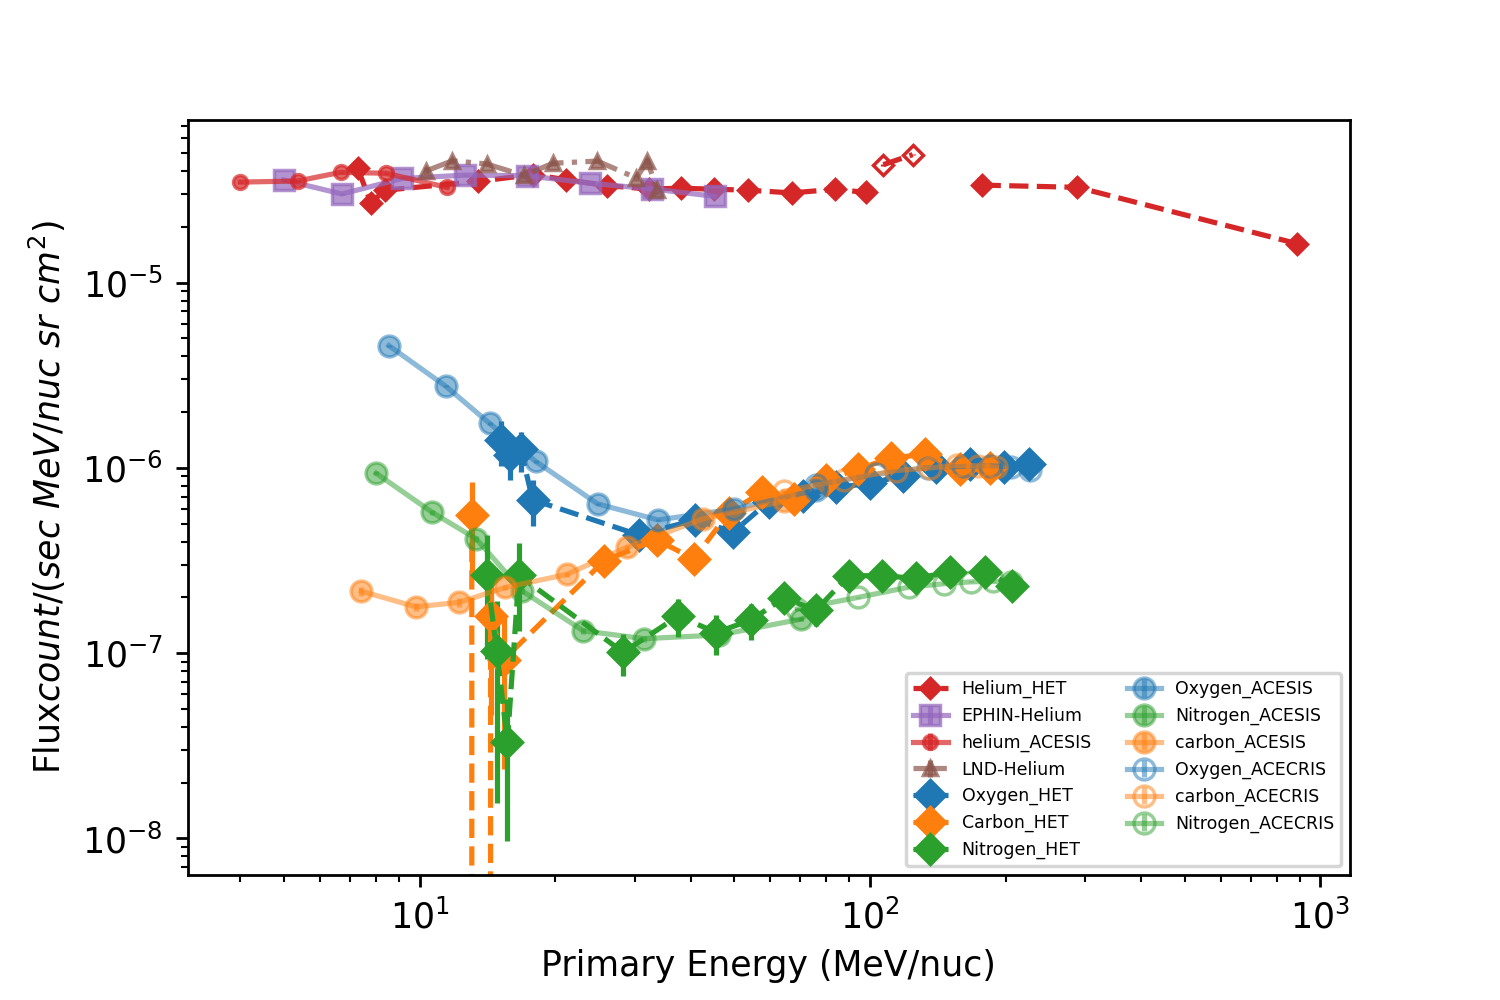
\includegraphics[width = 0.8\textwidth]{images/ACR/ACE_SIS_CRIS_SOLO_all_3.png}
    \caption[The quite time spactra of helium, carbon, nitrogen and oxygen between 2020 and 2022]{The helium-4 (red, brown, purple), carbon (orange), nitrogen (green) and oxygen (blue) spectrum averaged between 2020 and 2022. The \ac{SEP} events are removed. The data used in this figure consist of observation from \ac{SolO}/\ac{HET}, \ac{SOHO}/\ac{EPHIN}, \ac{ACE} and \ac{LND}}
    \label{fig:overview}
\end{figure}
\begin{figure}[!htb]
    \centering
    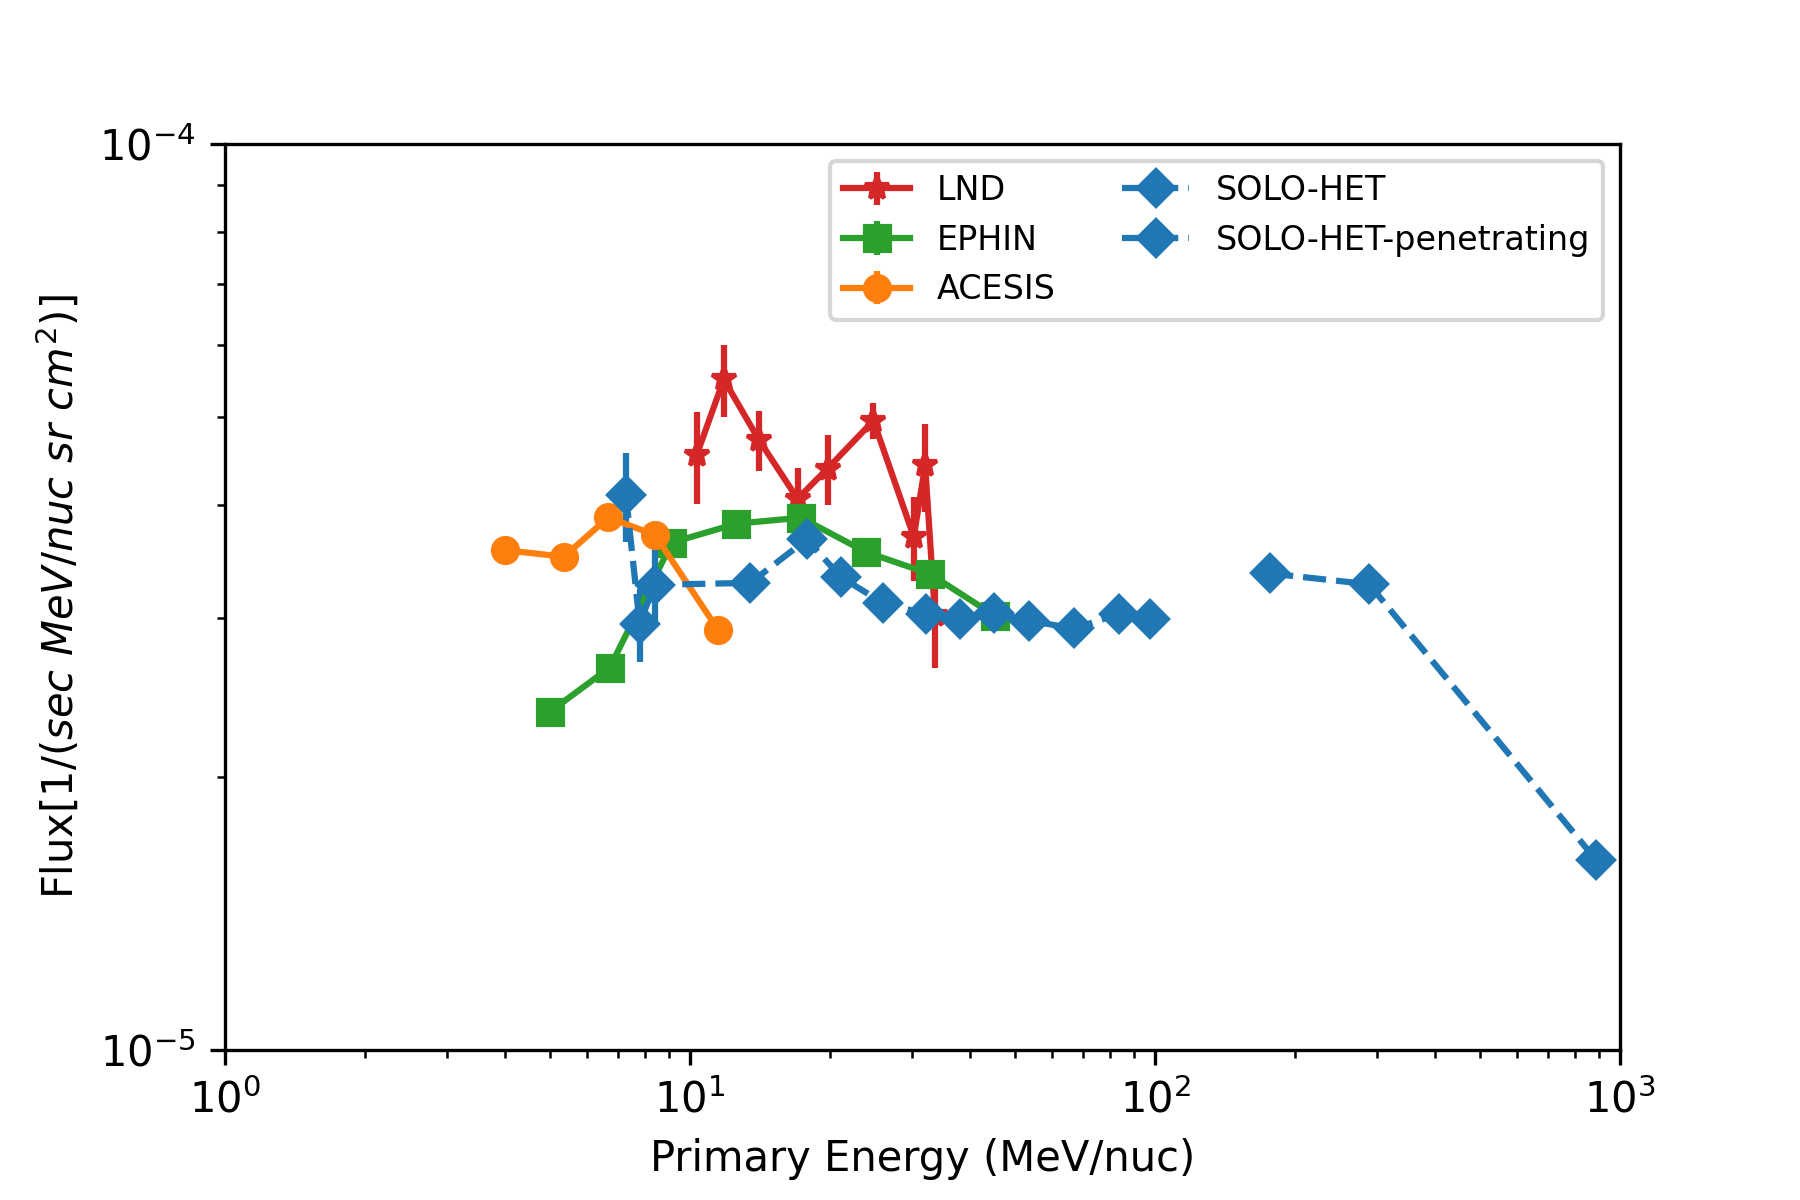
\includegraphics[width = 0.8\textwidth]{images/ACR/1AU_comparison_ACE_EPHIN_SOLO_SEP_version2.png}
    \caption[The helium spectra during the period \ac{SolO} between 0.95 and 1 au]{The helium-4 spectra of \ac{SolO}/\ac{HET}, \ac{SOHO}/\ac{EPHIN}, \ac{ACE}/\ac{ACESIS} and Chang'4/\ac{LND} when SOLO was between 0.95 and 1AU. The \ac{SEP} events are removed.}
    \label{fig:helium_spec_1au}
\end{figure}

\subsection*{Temperal variation of helium-4 intensity}

Fig.~\ref{fig:overview_helium_intensity} presents the intensity profile of helium from Feb 2020 to October 2022 on the reconstructed energy channels from \ac{HET}, \ac{EPHIN}, \ac{LND} and \ac{STEREO}-A. The energy range of recontructed channels are labeled as legends correspondingly. In the bottom panel, we again plot the variation of \ac{SolO} orbit distance.

It is evident from Fig.~\ref{fig:overview_helium_intensity} that from 2020 to the middle of 2021, the flux of helium-4 of energy below 50 MeV/nuc are generally dominated by the \ac{ACR} background.
only a limited number of large \ac{SEP} events occured at the end of 2020 \cite{Kolhoff2021AA}. After that,due to the increase of solar activities, the frequency of \ac{SEP} is noticeably increased, as shown in Fig.~\ref{fig:overview_helium_intensity} and Fig.~\ref{Fig:SOHO_EPHIN_Proton_flux}.
Those large and intense \acp{SEP} significantly disturbe the time profile of the \ac{ACR} background and consequently, we must remove them before calculating the \ac{ACR} radial gradient. 
Of note, the energetic helium arrive differently at \ac{SolO}, \ac{EPHIN} and \ac{STEREO}-A, and the discoutinuities of \ac{LND} measurements are due to the hibernation of \ac{LND} during local night on the Moon far-side surface.

In addition to the intermittent occuring \ac{SEP}, the long-term decrease is also clear shown in the \ac{SolO} and \ac{EPHIN} time profiles from 2020 to the end of 2022. This is because of the enhanced solar modulation of cosmic rays. The interplay between the large scale \ac{HMF} significantly reduce the number of \acp{ACR} arrival at the Earth and further the inner heliosphere below 1 au. We could foresee the further decrease of the \ac{ACR} intensity in the new few years before the solar acitivity reach the maximum in 2025 \citep{}.

In contrast to the transient variation from \ac{SEP} and 11-year variation due to the large-scale solar modulation, the intensities of cosmic rays are also influenced and modulated by recurring, compressed structures that are formed from the interaction between fast and slow solar wind stream emitted from the solar surface. Such structures enhance the pressure and density of plasma and corotate with the Sun periodically with a period of approximately 27 days. Hence we call them stream interaction regions or corotating interaction regions \citep{Burlaga1974JGR, Gosling1976JGR, Richardson2004SSRv}. The changes of local conditions modify the transport of cosmic rays, resulting intensity changes though are not as significant as those due to \acp{SEP} and solar modulations.

\begin{figure}[!htb]
    \centering
    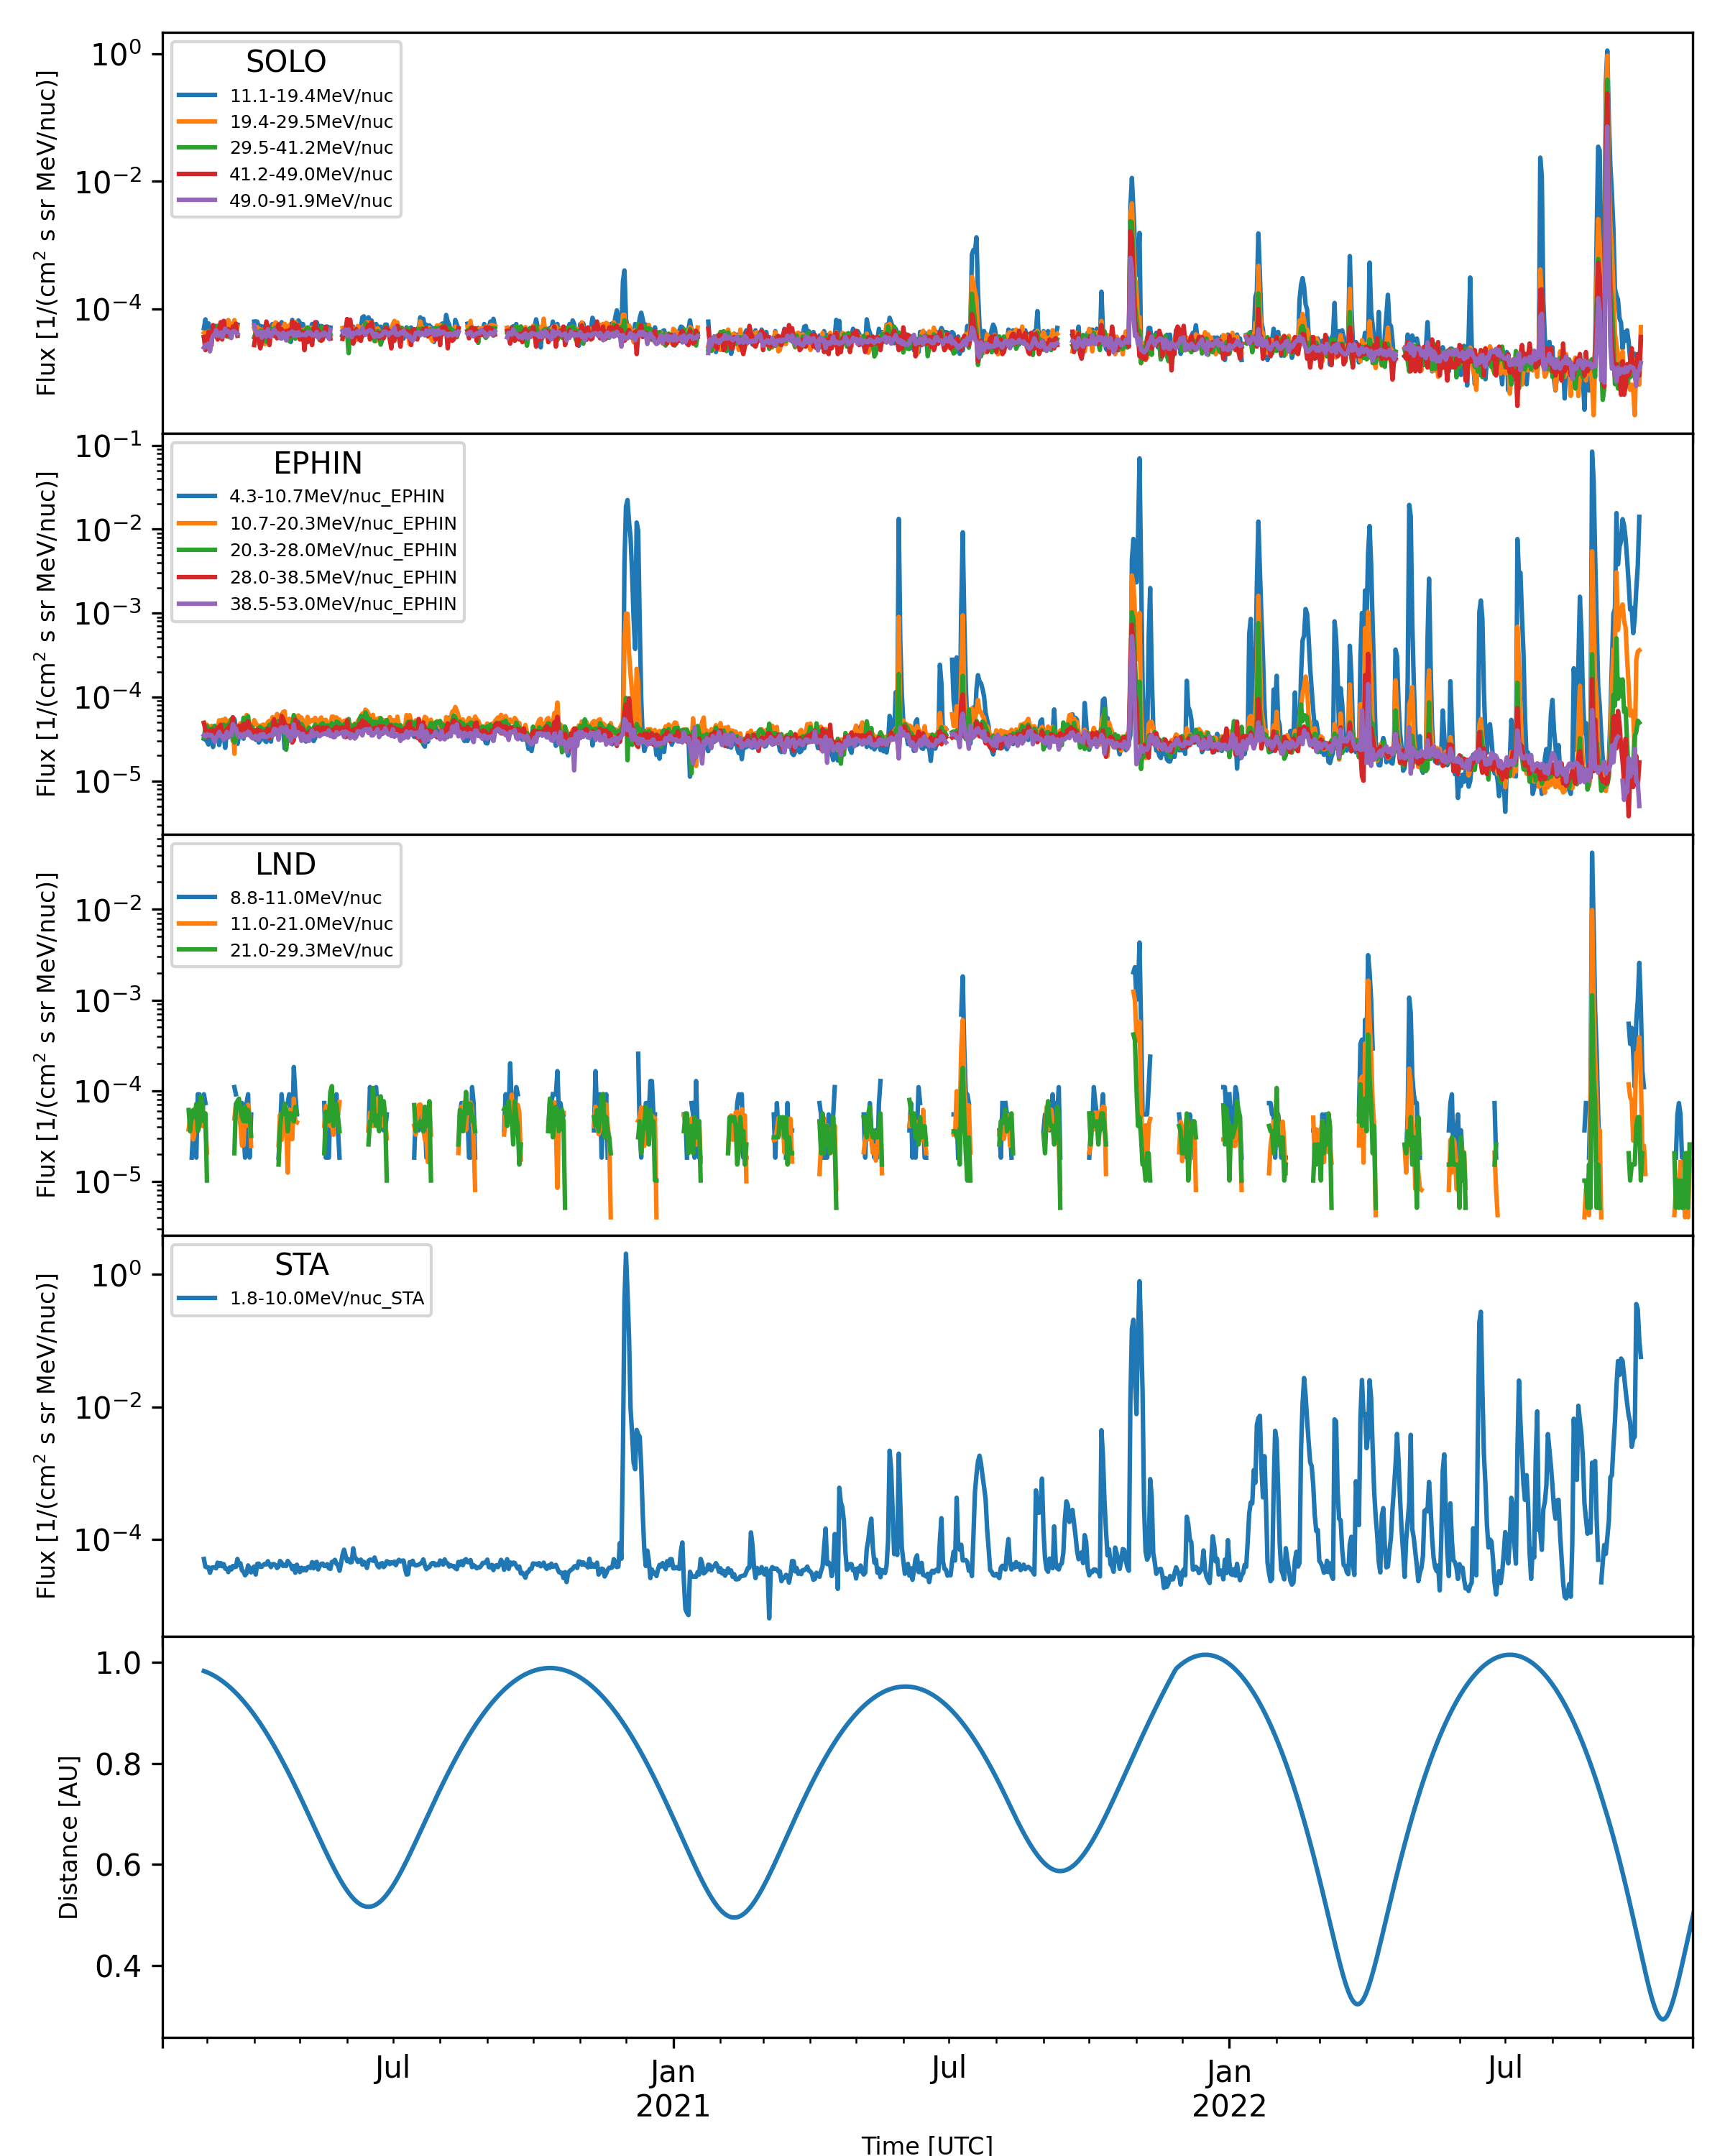
\includegraphics[width = 0.8\textwidth]{images/ACR/overview_Helium_4_instrument.png}
    \caption[Overview of the helium measuremet by different instruments]{From top to the bottom: The daily averaged helium flux measured by \ac{SolO}/\ac{HET}, \ac{SOHO}/\ac{EPHIN}, Chang'E-4/\ac{LND}, and \ac{STEREO}-A/\ac{LET} over 2020.2 - 2022.10. The bottom plot shows the radial distance of \ac{SolO} away the sun.
    %The red dashed lines indicate the SEP events that we determined by eye.
    \TODO{reminder: you should better re-load the SOLO data, and check the isotropic between different direction, and resample data before further process like sum all direciton or somesome.}}
    \label{fig:overview_helium_intensity}
\end{figure}




\begin{table}[!htb]
    \centering
	\caption[Time perods \ac{SolO} closed to 1 au]{A list of time perods when the solar radial distance of \ac{SolO} is between 0.95 and 1 AU. The distance between \ac{SolO} and Earth is also given.}
	\label{tab:1AU_period}
    \begin{tabular}{|c|c|c|c|}
    \hline
	periods & start time & end time & distance to Earth  (au)\\
    \hline
    1   & 2020-02-28 & 2020-03-16   & 0.07 \\
    \hline
	1	& 2020-09-14 & 2020-11-10	& 1.76 \\
    \hline
	2	& 2021-05-27 & 2021-06-09	& 1.49 \\
    \hline
	3	& 2021-11-21 & 2022-01-15	& 0.13 \\
    \hline
	4	& 2022-06-05 & 2022-08-02	& 1.96 \\
    \hline
    5 (not used)	& 2023-01-04 & 2023-01-17	& 0.41 \\
    \hline
    \end{tabular}
\end{table}

\section{Averaged helium intensity profile}
\subsection*{Solar energetic particle events list}

As we aforementioned, \ac{SEP} is one of most manifest disturbance to the \ac{ACR} background. Therefore, a completed and properly defined \ac{SEP} periods are crucial. In this section we explain what type of data we used and how we determine the \ac{SEP} periods.Because \ac{SEP} arrived differently at \ac{SolO} and at the Earth. Therefore the \ac{SEP} list are determined seperated for both cases.

In order to remove the solar particle thoroughly and prevent the existence of remanent particles that could not be recognized directly from the intensity profiles, we consider utilizing different data products to identify the \acp{SEP} rather than based on the helium data.

Fig.~\ref{Fig:solo-lvl2} presents the 10-minute count rate of L2 counter which are named as HET\_any(a1, b1) and HET\_any(a2, b2), the former from the sunward telescope and the latter from the anti-sunward telescope. As we explained in the instrument section, those channels are perfect indicators of the \ac{SEP} with larger counting statistics, approximately 600 per ten minutes. Since the profile of both case are similar, we only use the sunward measurement for the determination of \ac{SEP} periods. The \acp{SEP} that reach the Earth are determined by the time profile of proton of energy below 10 MeV that were observed by \ac{EPHIN}.

The duration of the SEP is simply determined by the 3-$\sigma$ method with the eye determination as supplements. $\sigma$ is the standard deviation of a background or the preevent quite time. The \ac{SEP} periods are defined as the consecutive time series when the flux is 3 time of the standard derivations above the background. This method was commonly used in determining the onset time of the SEPs event and valid for those SEPs has clear onset and sharp increase. 
However, if the background is unclear and increase of the temporal profiles is slow, the determination of the onset and end of event might have larger uncertainty. In this case, we determine the boundary of periods by eye.

As a result, the \ac{SEP} periods that we determined are illustrated as the magenta color region in Fig.~\ref{Fig:solo-lvl2} and Fig.~\ref{Fig:SOHO_EPHIN_Proton_flux}, and the \ac{SEP} periods are listed in Table.~\ref{tab:solo_SEPlist} and \ref{tab:SOHO_SEP_list} in Appendix {chp:SEPlist}.



\begin{figure}
    \centering
    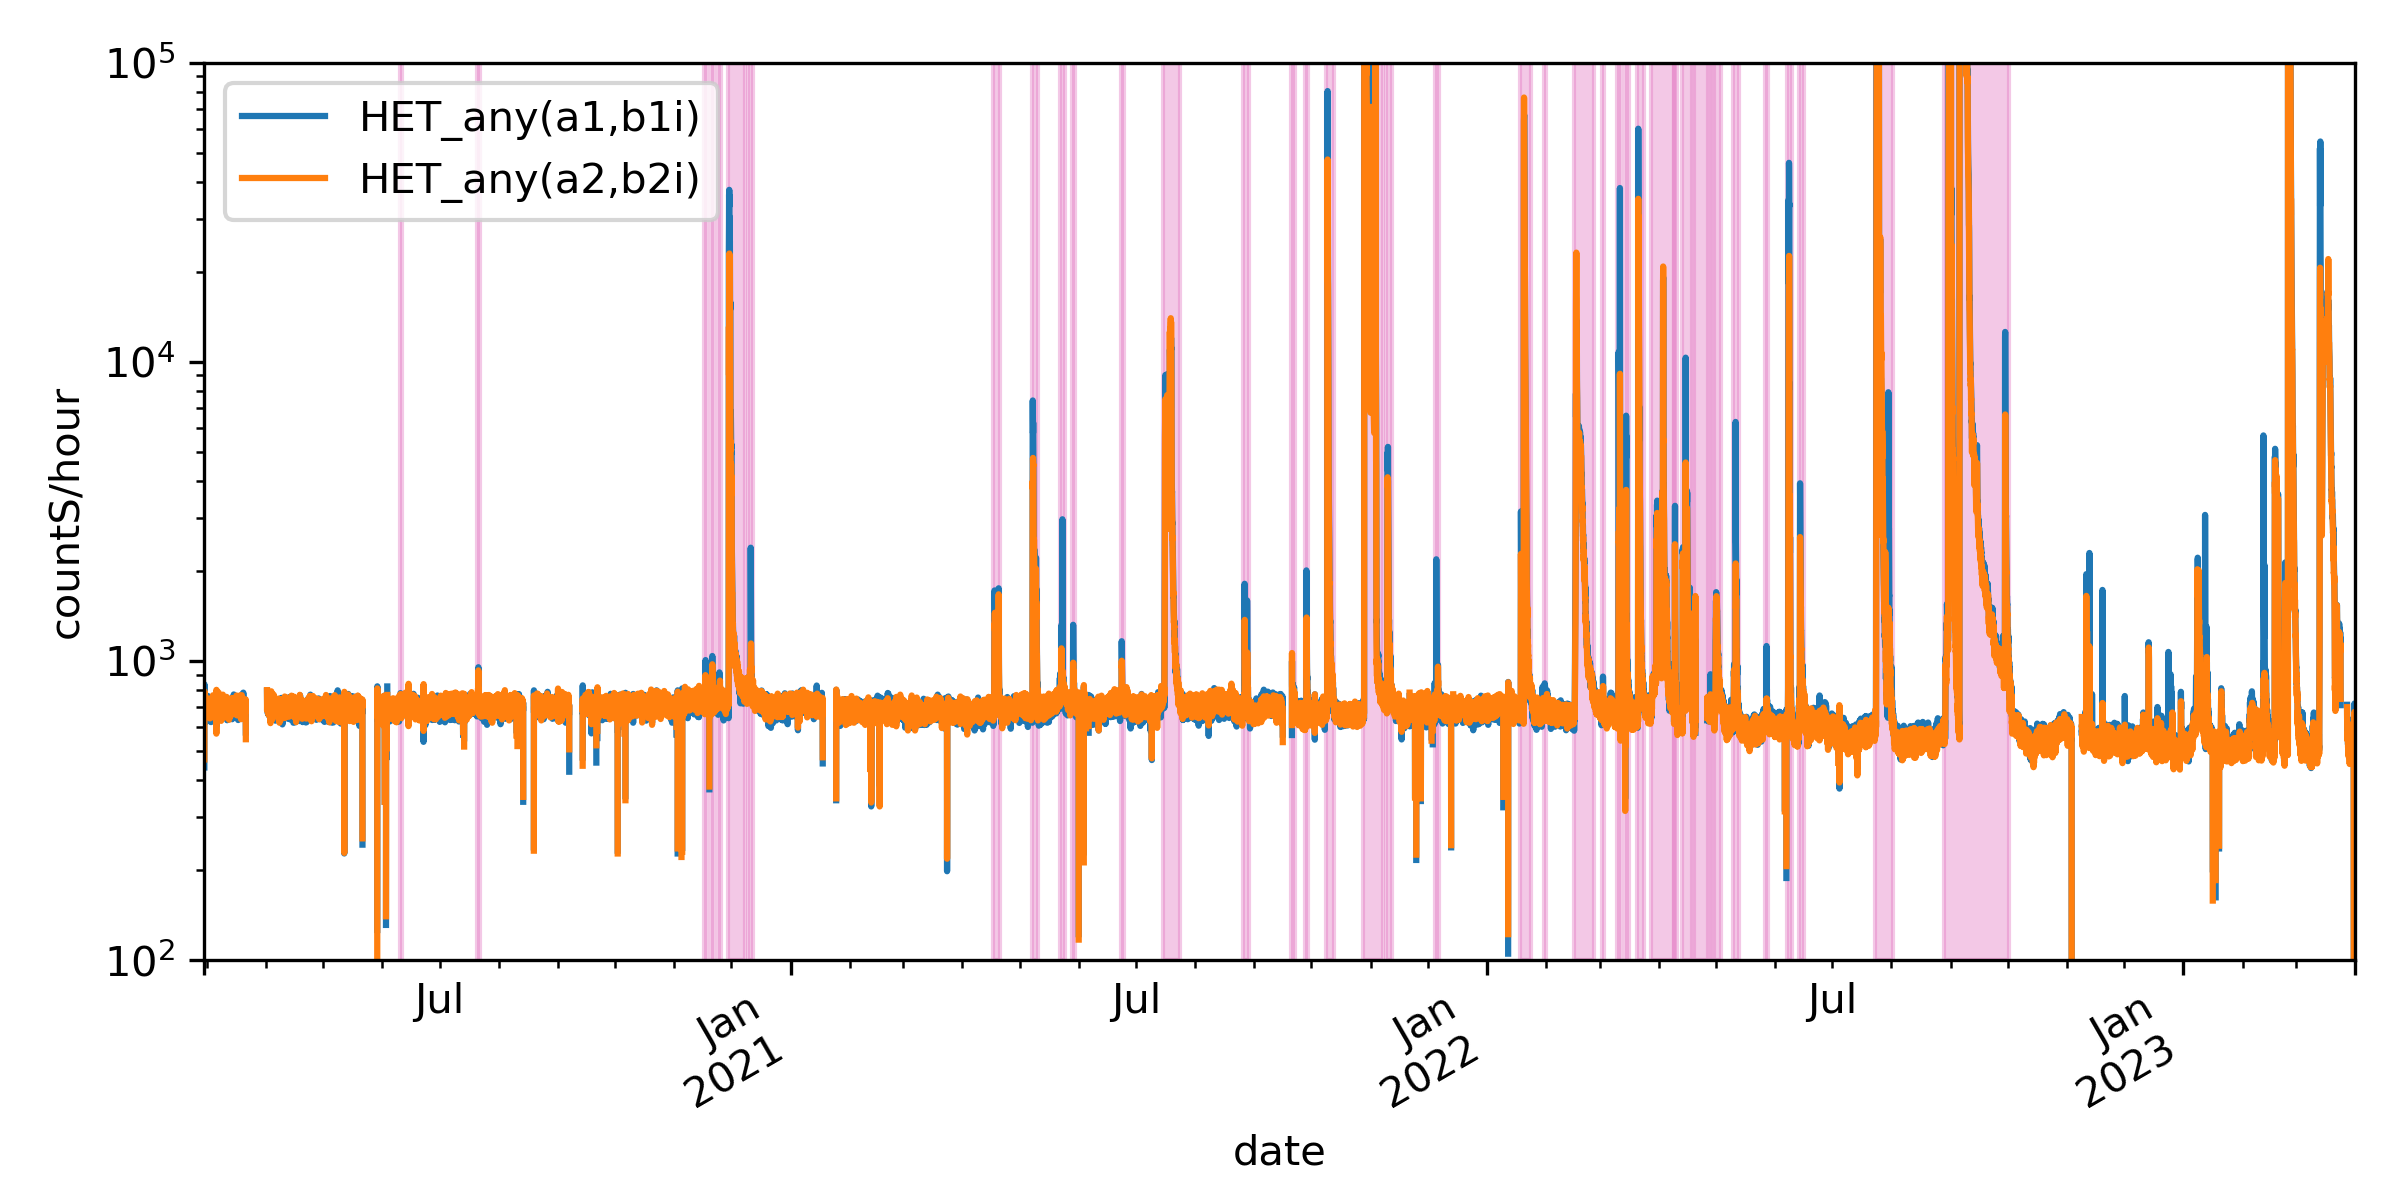
\includegraphics[width = \textwidth]{images/ACR/SOLO-lvl2-trriger.png}
    \caption[The L2 counter of \ac{HET}]{The Level-2 counter of the \ac{HET} named any(a1,b1) and any(a2,b2). The magenta color regions are the SEP periods we identified.}
    \label{Fig:solo-lvl2}
\end{figure}



\begin{figure}[!htb]
    \centering
    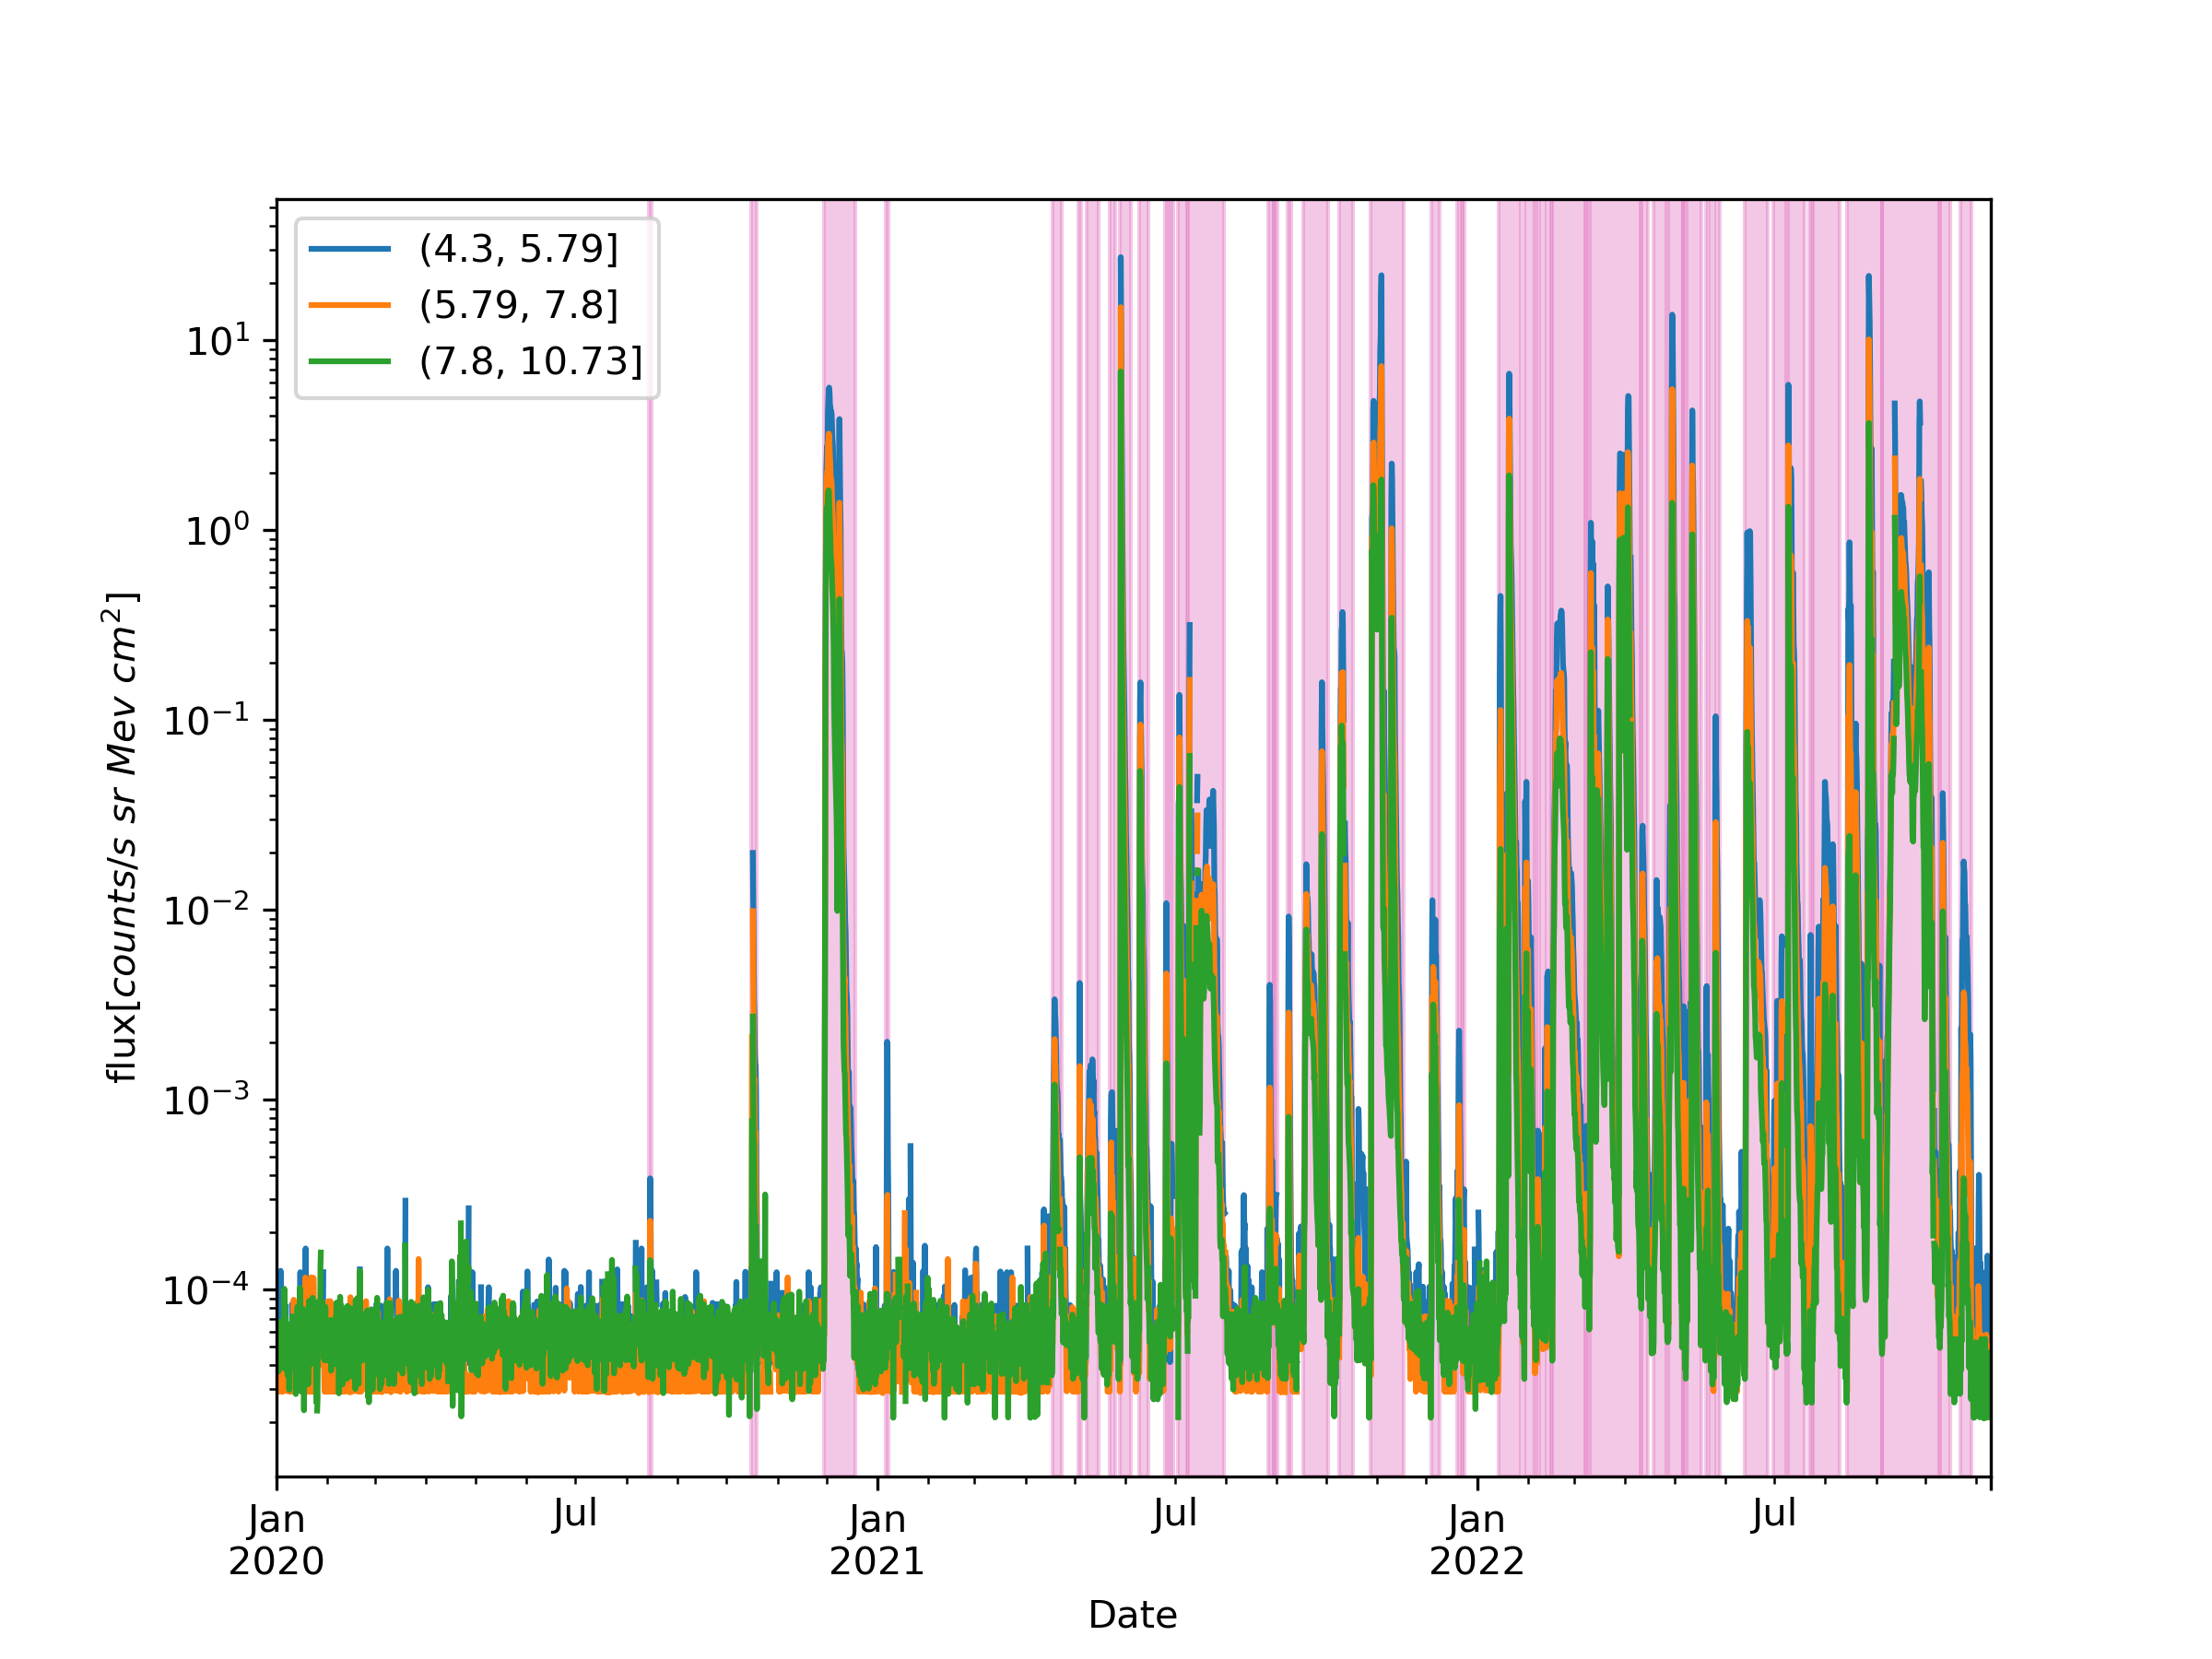
\includegraphics[width = \textwidth]{images/ACR/SOLO-EPHIN-l3i-log2+6-proton-6H.png}
    \caption{The intensity profile of proton of energy below 10 MeV}{The proton flux measured by SOHO/EPHIN below 10 MeV. The data we used here are the level-3 proton data products. The magenta shadow regions are the SEP.}
    \label{Fig:SOHO_EPHIN_Proton_flux}
\end{figure}

\subsection*{Averaged over Carrington rotation}

As mentioned earlier, transient \acp{SEP}, long-term solar modulation, and periodic \ac{CIR} and \ac{SIR} significantly affect the \ac{ACR} intensity. In the previous section, we have identified and removed \ac{SEP} periods, obtaining a slowly changed profile. In this section, we will further reduce the impact of recurring compressed regions by averaging the intensity profile over the carrington rotation. The carrington rotation is defined in the second panle from top in Fig.~\ref{fig:SOLO_orbit_info} which illustrate the the carrington longititude of \ac{SolO}. It is worth noting that the length of a carrington rotaion in the \ac{SolO} corrdinate varies as the spacecraft moving closer to and further away from the sun. 

Fig.~\ref{fig:carrington_flux} displays the averaged helium flux from \ac{HET} (orange line) and \ac{EPHIN} (blue line). The red dashed lines indicate the variation in radial distance between \ac{SolO} and the sun. Despite the approximately 30\%/au radial gradient \citep{Rankin2021ApJ} that we expect and the slight discrepancy of the energy channels between \ac{HET} and \ac{EPHIN}, the measurements show overall consistency for all the four channels, even though the flux decrease over time. The decreases in the flux is significant and is modulated by the sun.

More interestingly, during the end of 2020 and start of 2021, the \ac{HET} helium intensity is unusualy higher than that of \ac{EPHIN}. The discrepancies are up to 30 \% and are clear seen in four channels. Though that data point is from a carrington rotation with an larger \ac{SEP} event, we have already removed the \ac{SEP} periods from the data. Besides, such an increase are even more clear in the higher energy channel (bottom panel). 

Furthermore, the bottom panel of Fig.~\ref{fig:carrington_flux} shows that before 2021, the intensities of 40 - 50 MeV/nuc helium from \ac{EPHIN} is statistically lower than that from \ac{HET}. After that, such a discrepancy is gradually disappeared in this channel. Besides, such a discrepancy is unseen in the lower energy channels and. Currently, the reasons for these discrepancise are unclear.

Fig.~\ref{fig:fluxvsdistance} shows how the flux of helium with energy range of 10 - 20 MeV/nuc from \ac{HET} change as a function of the radial distance from 0.4 to 1 au. Averaged fluxes of four orbits are showed in different colors, as the legends indicate. And the blue triangles overlaid solid circles suggest the time order of measurements. The intensity of helium of the last measurement is about 5 times less than that of the begnning. Obviously, we could not derive the actual radial gradient from this plot directily.


\begin{figure}
    \centering
    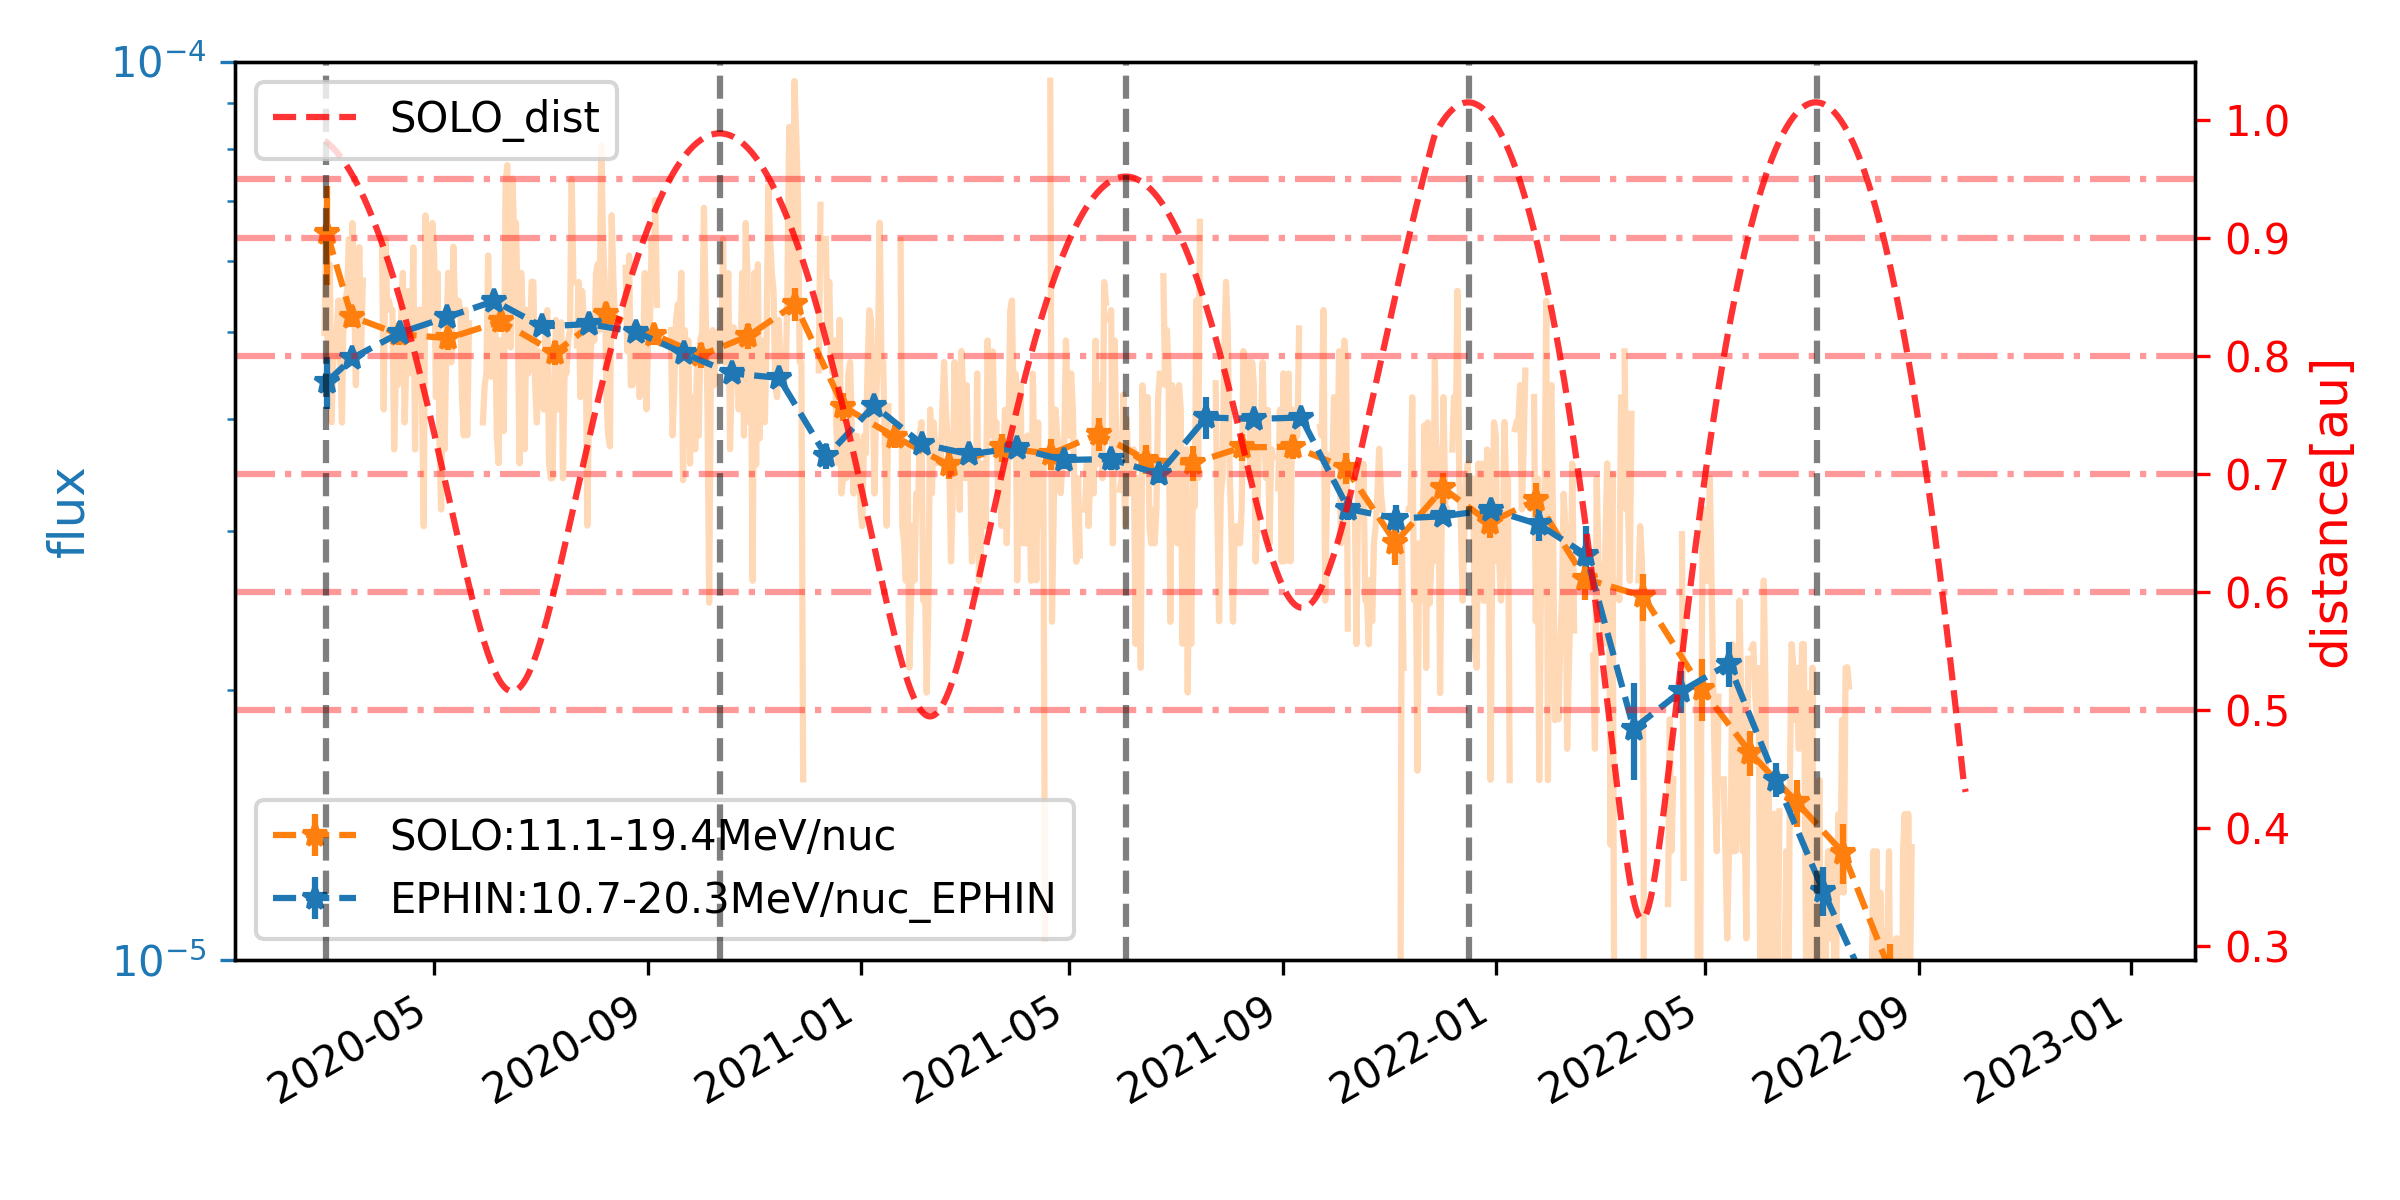
\includegraphics[width = 0.8\textwidth, height = 0.2\textheight]{images/ACR/seperate_mask_1-3_newSOHOSEPmask/Carrington_SOLO_11.1-19.4MeV_EPHIN_10.7-20.3MeV.png}
    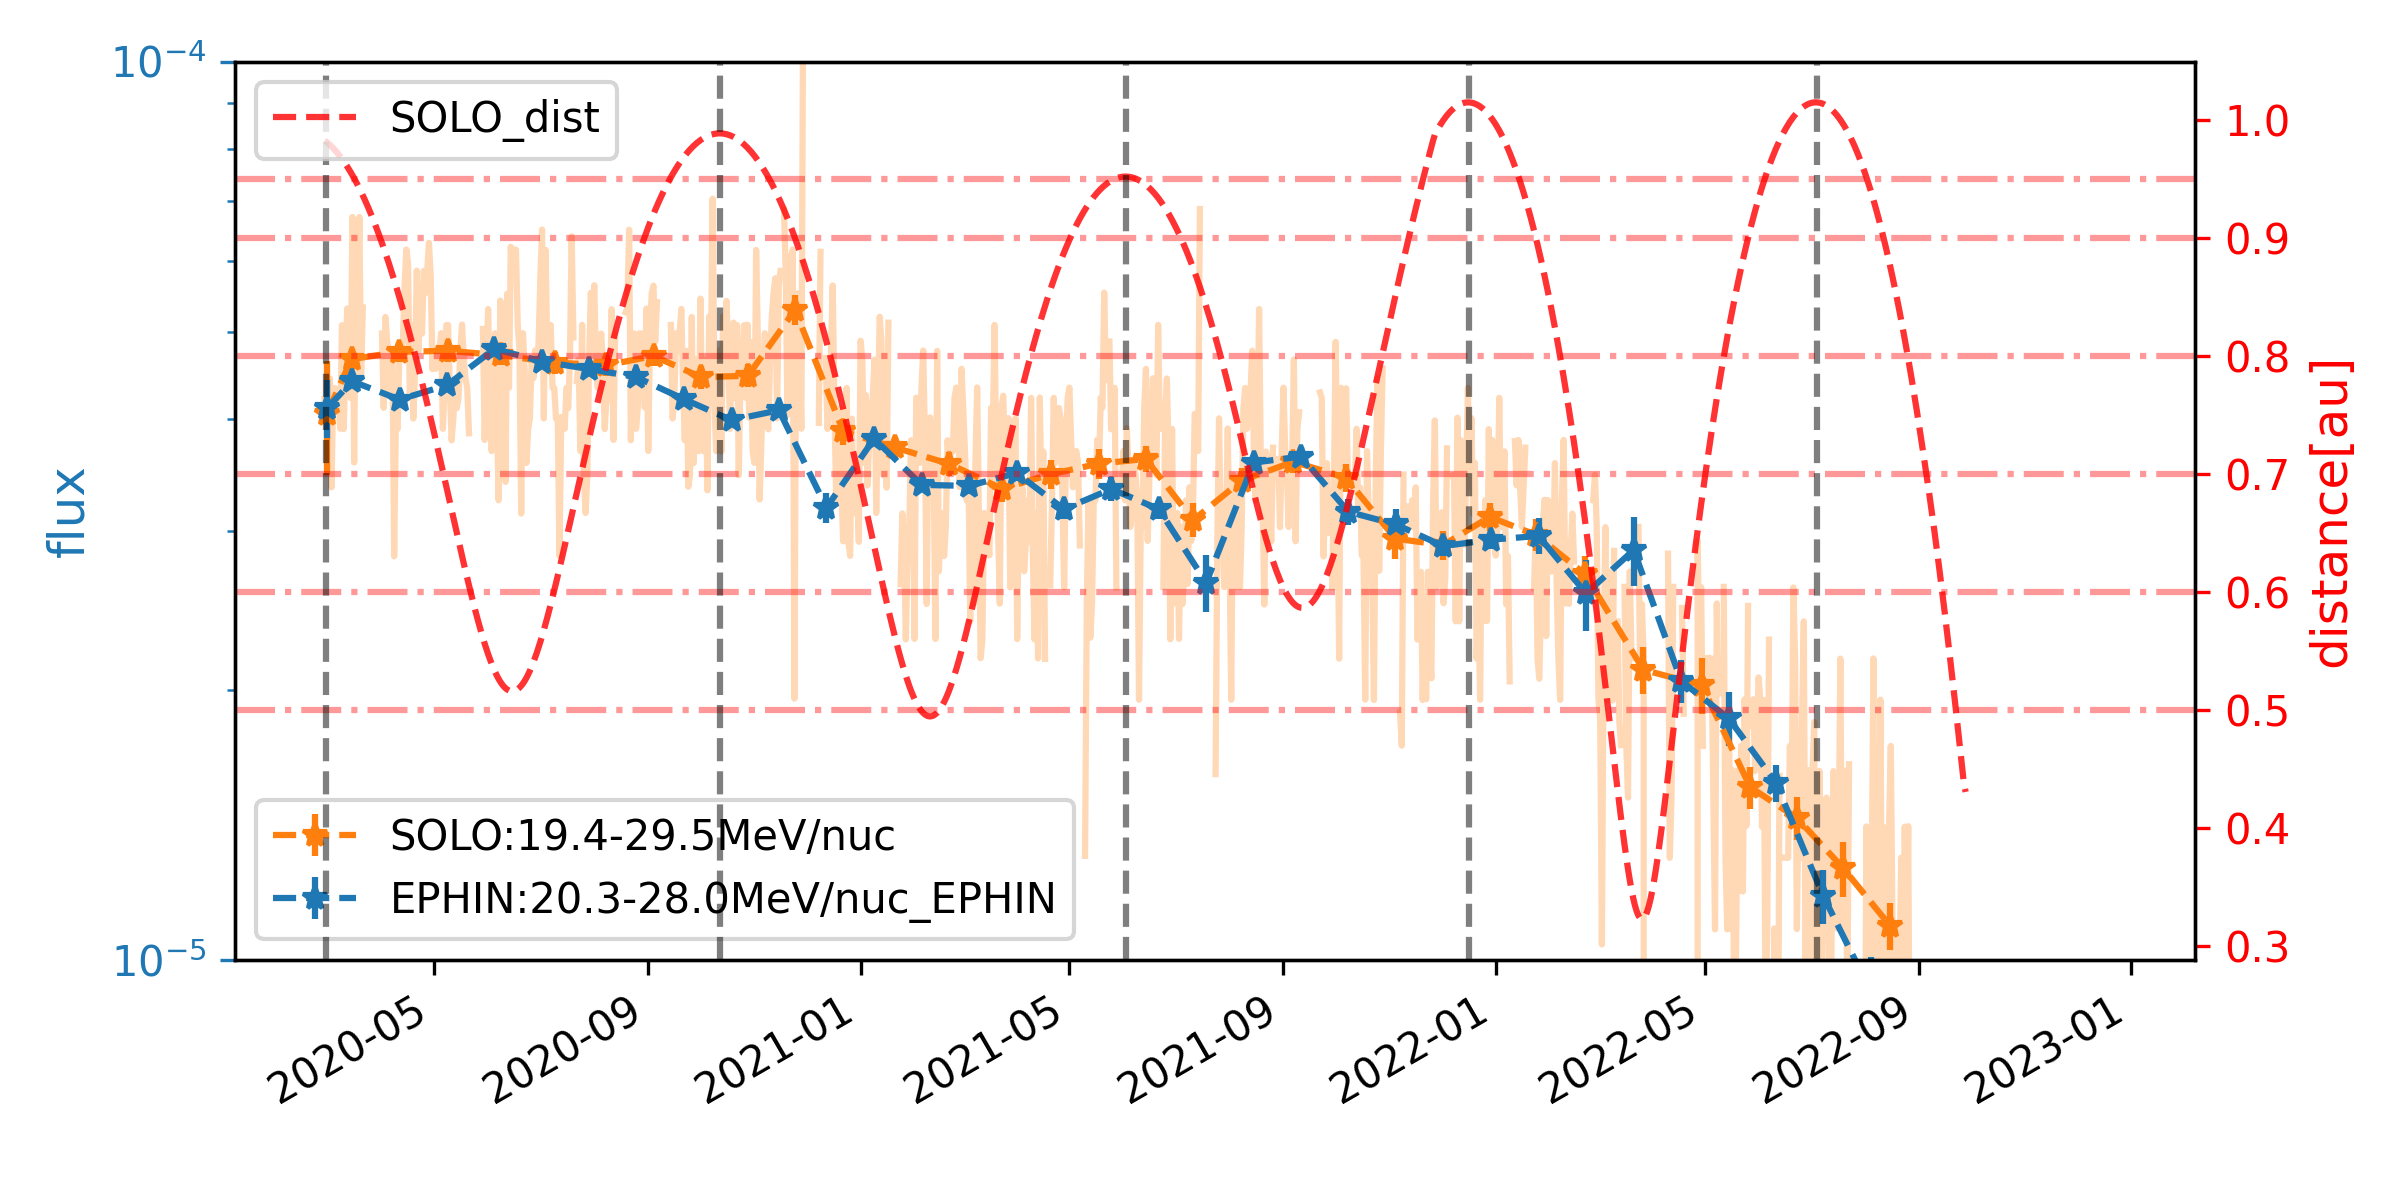
\includegraphics[width = 0.8\textwidth,height = 0.2\textheight]{images/ACR/seperate_mask_1-3_newSOHOSEPmask/Carrington_SOLO_19.4-29.5MeV_EPHIN_20.3-28.0MeV.png}
    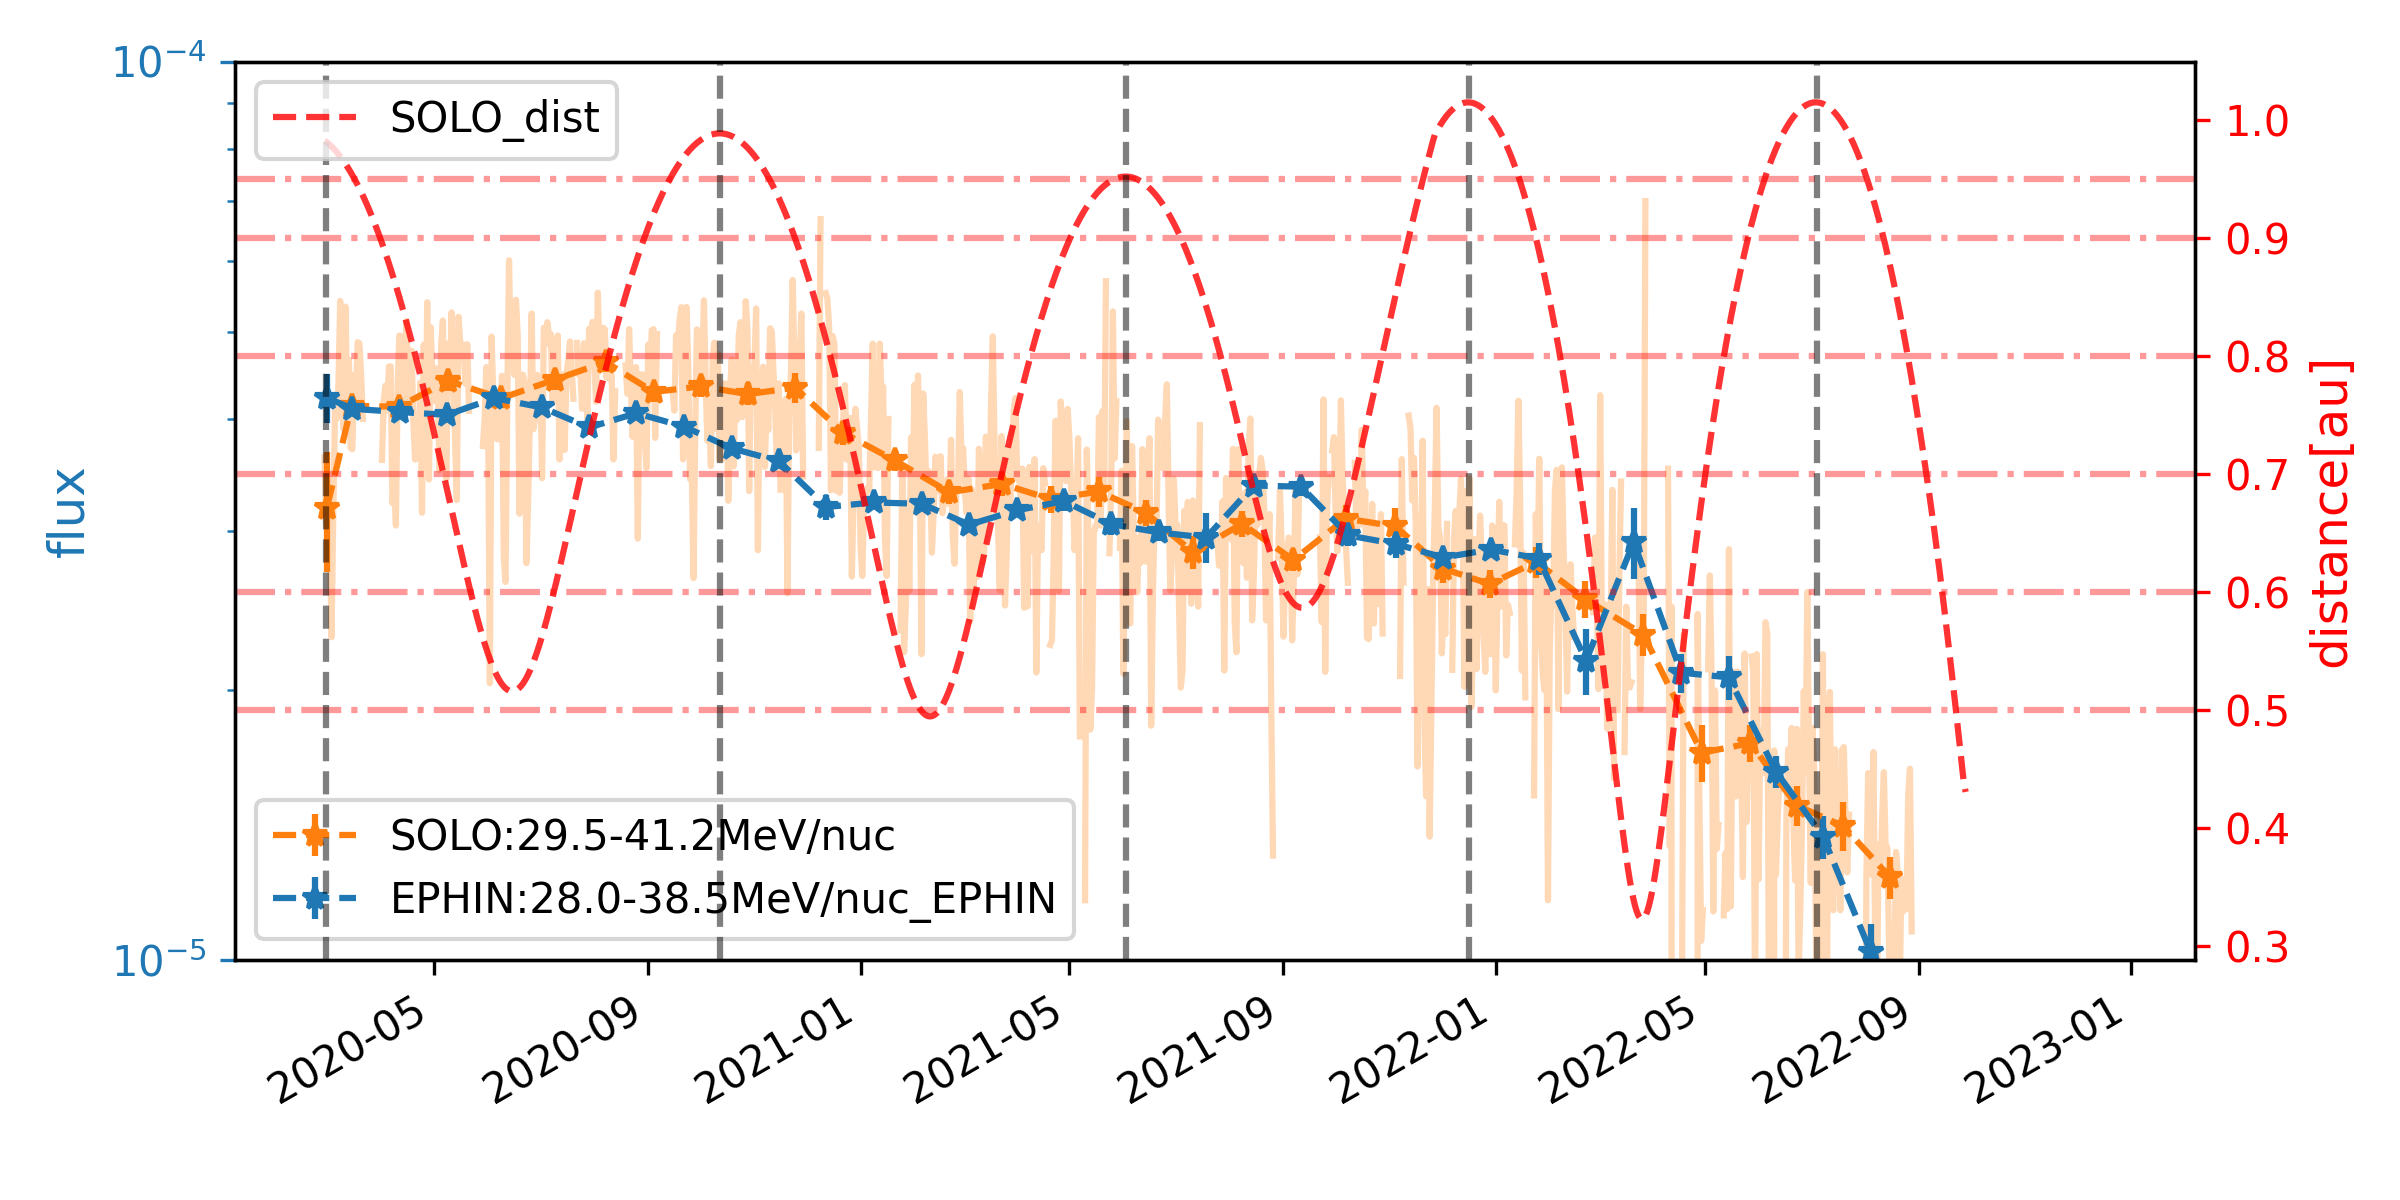
\includegraphics[width = 0.8\textwidth,height = 0.2\textheight]{images/ACR/seperate_mask_1-3_newSOHOSEPmask/Carrington_SOLO_29.5-41.2MeV_EPHIN_28.0-38.5MeV.png}
    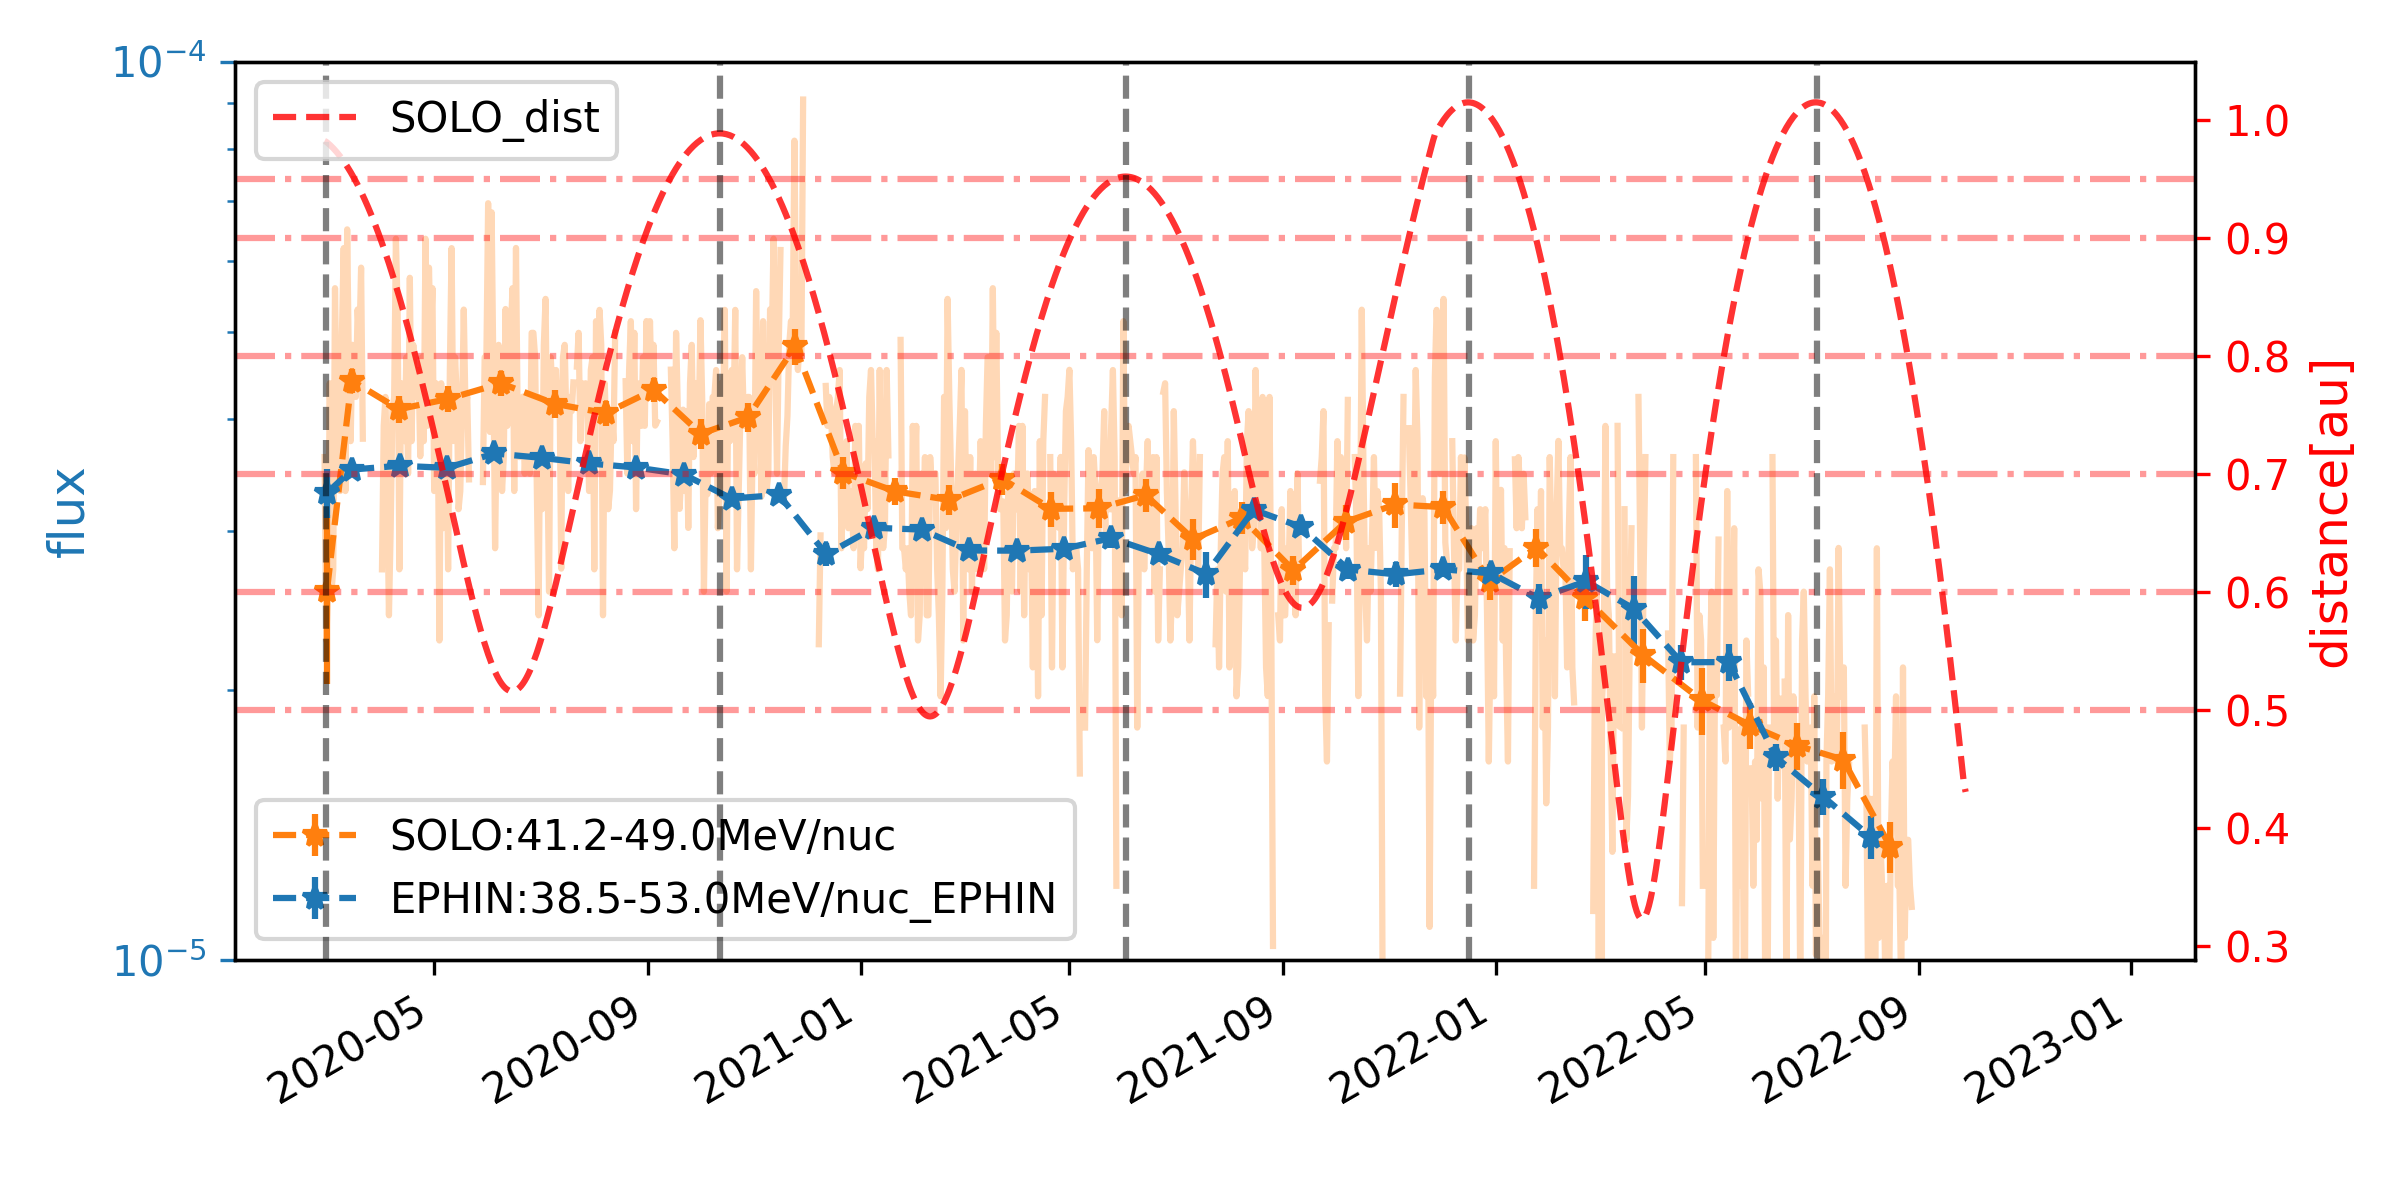
\includegraphics[width = 0.8\textwidth,height = 0.2\textheight]{images/ACR/seperate_mask_1-3_newSOHOSEPmask/Carrington_SOLO_41.2-49.0MeV_EPHIN_38.5-53.0MeV.png}
    \caption[The helium flux averaged over the the carrington rotation periods in four energy channels between 10 and 50 MeV/nuc]{The flux of \ac{SolO} (orange) and \ac{EPHIN} (blue) averaged over the carrington rotation periods in the energy channels of 10 - 20 MeV/nuc, 20 - 30 MeV/nuc, 30 - 40 MeV/nuc and 40 - 50 MeV/nuc. The daily averaged \ac{HET} helium flux, as indicated by the fluctuatign light orange lines, is also shown for different energy channels. Red dashed lines are the radial distance of \ac{SolO} to the sun.}
    \label{fig:carrington_flux}
\end{figure}

\begin{figure}
    \centering
    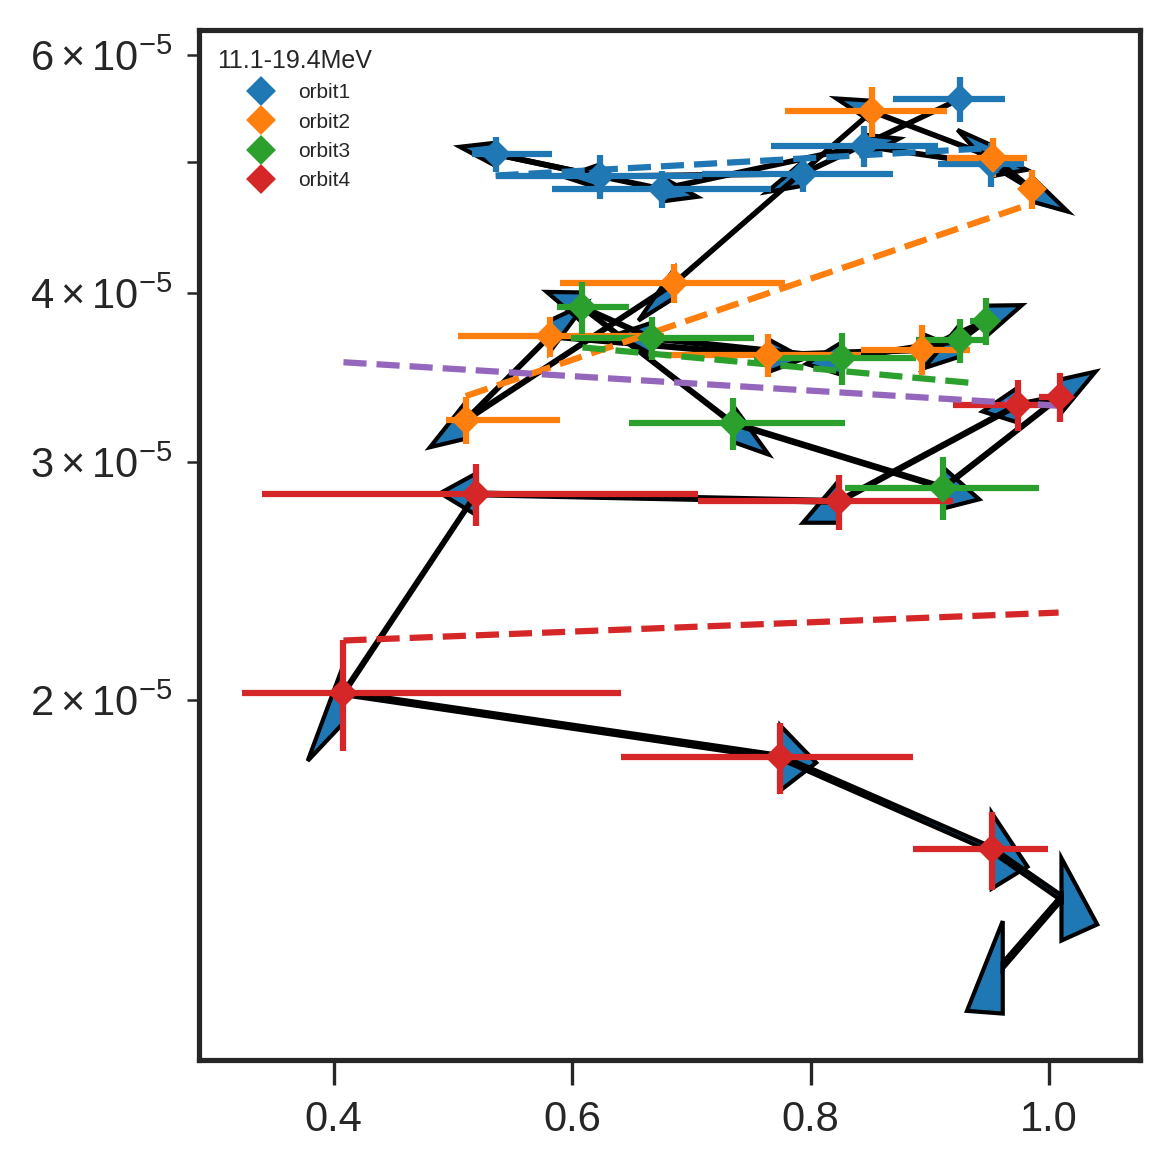
\includegraphics{images/ACR/SOLO-flux_only.png}
    \caption[10 - 20 MeV/nuc \ac{HET} helium flux vs the radial distance of \ac{SolO}]{The flux of 10 - 20 MeV/nuc helium from \ac{HET} changes a function of the radial distance of \ac{SolO}. The data from different orbit are show in different colors. The arrow indicates the direction of time.}
    \label{fig:fluxvsdistance}  
\end{figure}


\section{Radial gradient of ACR helium}

Deriving the limited radial gradient from the substantially changed data are challenging, in particular, under the case that the 5-fold decrease of the helium intensity caused by the solar modulation.
Therefore, in order to obtain the radial gradient, we de-trend the \ac{HET} flux by using the \ac{EPHIN} flux as baselines. By assuming the solar modulation is the same for both instruments, we first calculate the ratio of \ac{HET} and \ac{EPHIN} and estimate the radial gradient of different energy \ac{ACR} helium following the defination in Eq.~\ref{eq:radial_gradient}

We present the variation of the \ac{HET} to \ac{EPHIN} ratio for four energy channels in panels in the first and third row of Fig.~\ref{fig:ratio_radialgradient}. Similary, the radial distance of the \ac{SolO} is also given in the orange line. The colored regions indicate the orbit periods. The corresponding log-linear fitting lines are given in the second and the forth row respectviely. The fiitted lines are shown as the dashed lines and the 95\% confident intervals are shown as shaded regions. Only the data points from first orbit to the third orbit are used for the fitting and shown seperately in different colors. The averaged radial gradients are fitted over the data of the first three orbits and shown as black dashed lines.
That is because the \ac{SEP} dominated the data in the forth orbit and most of data are removed, causing the larger uncertainties in the fitting. The radial gradient of helium in different energy channels at different orbit are given in Table~\ref{Tab:radialgradient_1}.



\begin{figure}[!htb]
    \centering
    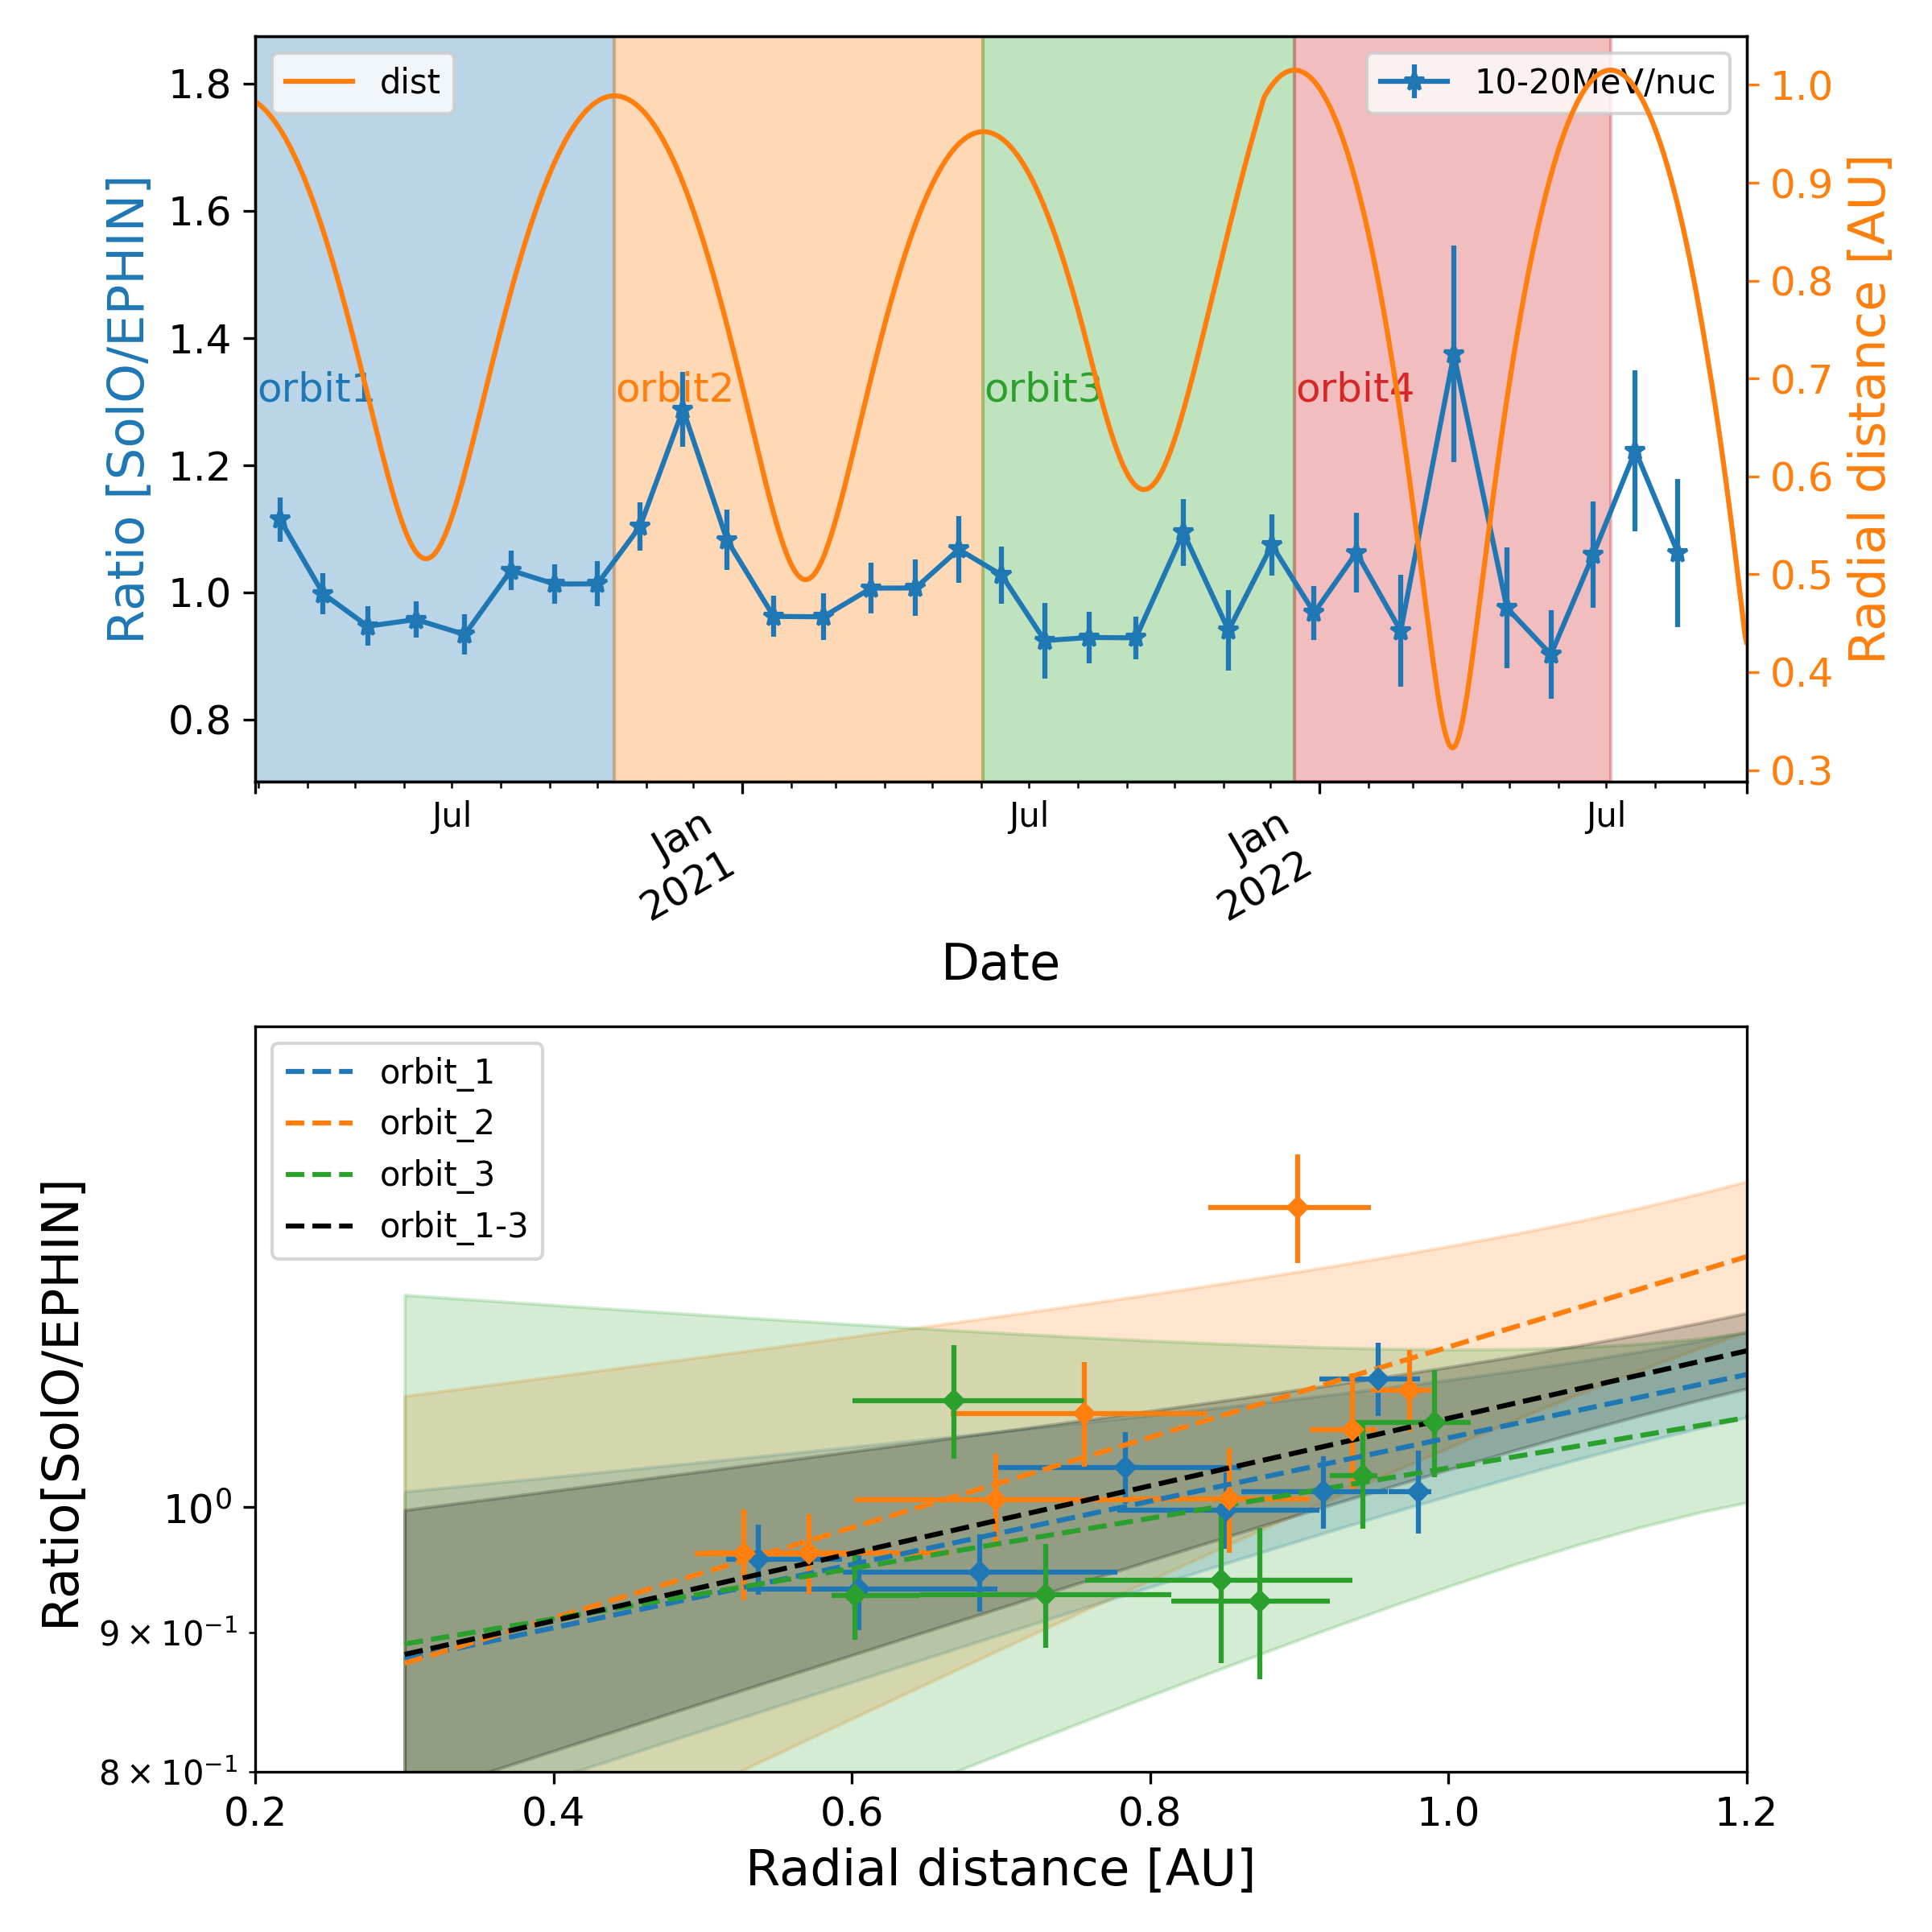
\includegraphics[width =0.48\textwidth, height = 0.3\textheight]{images/ACR/seperate_mask_1-3_newSOHOSEPmask/ratio_time_radialgradient_10-20MeV.png}
    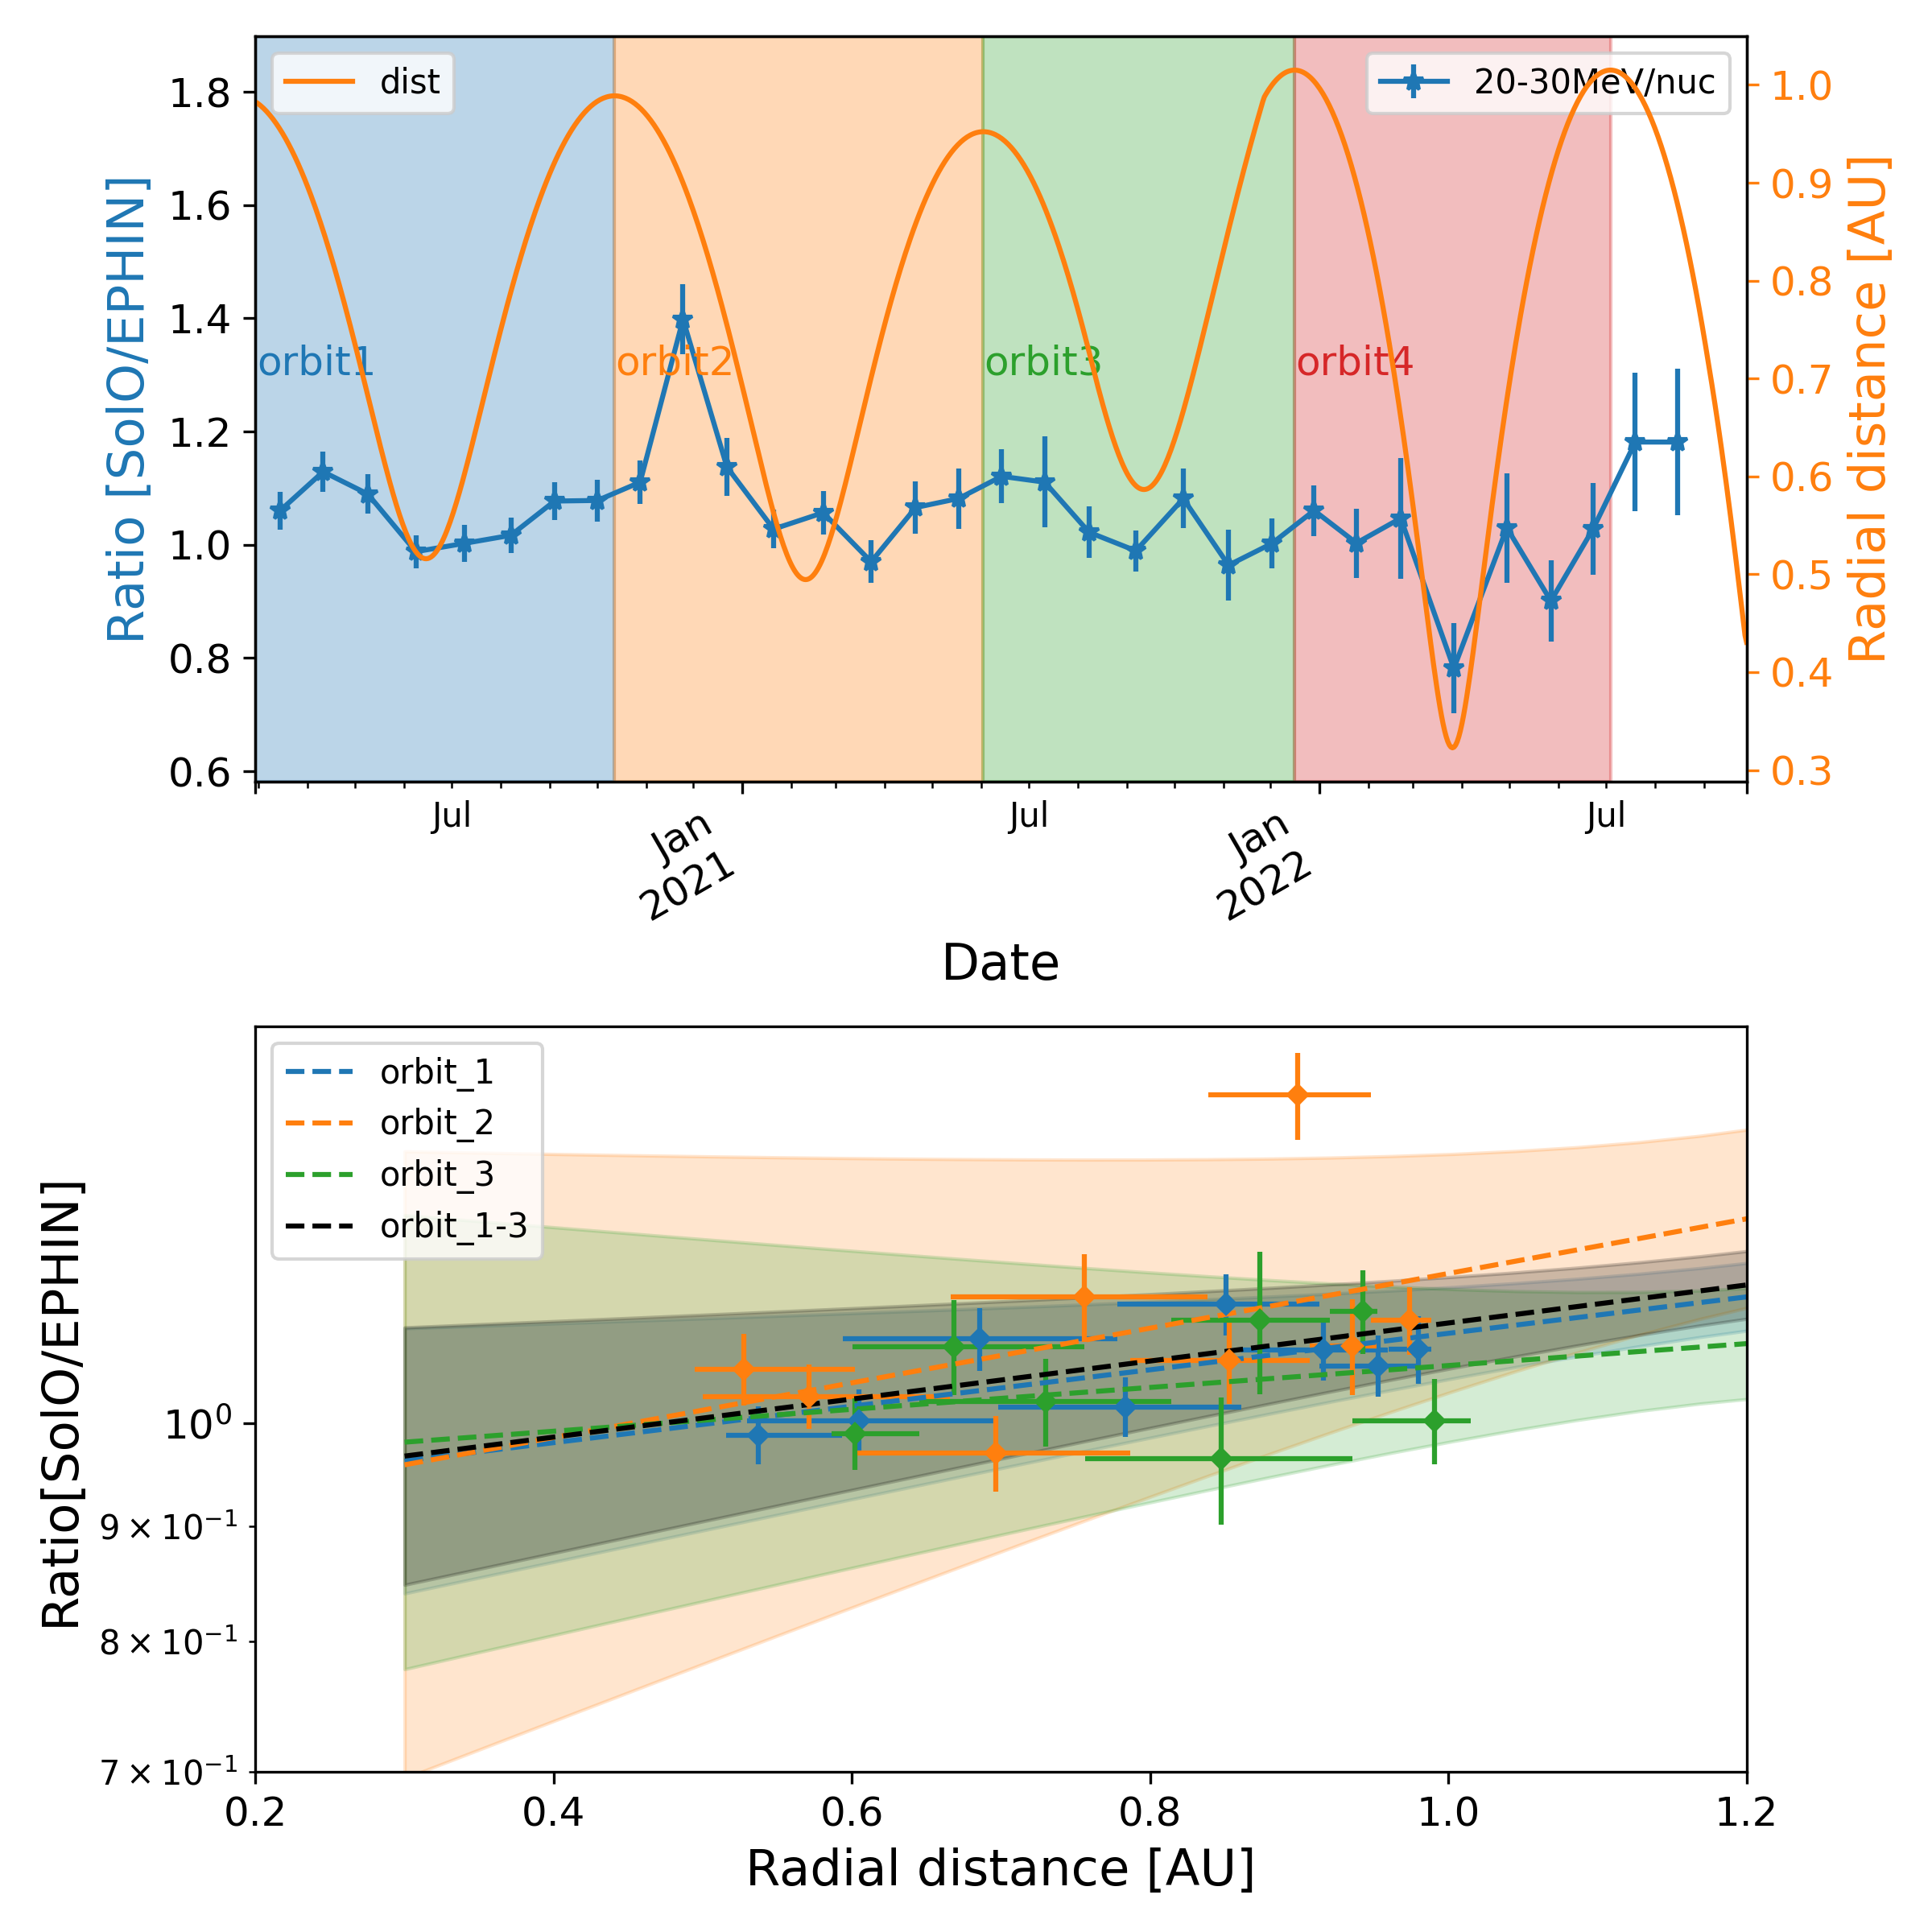
\includegraphics[width =0.48\textwidth, height = 0.3\textheight]{images/ACR/seperate_mask_1-3_newSOHOSEPmask/ratio_time_radialgradient_20-30MeV.png}
    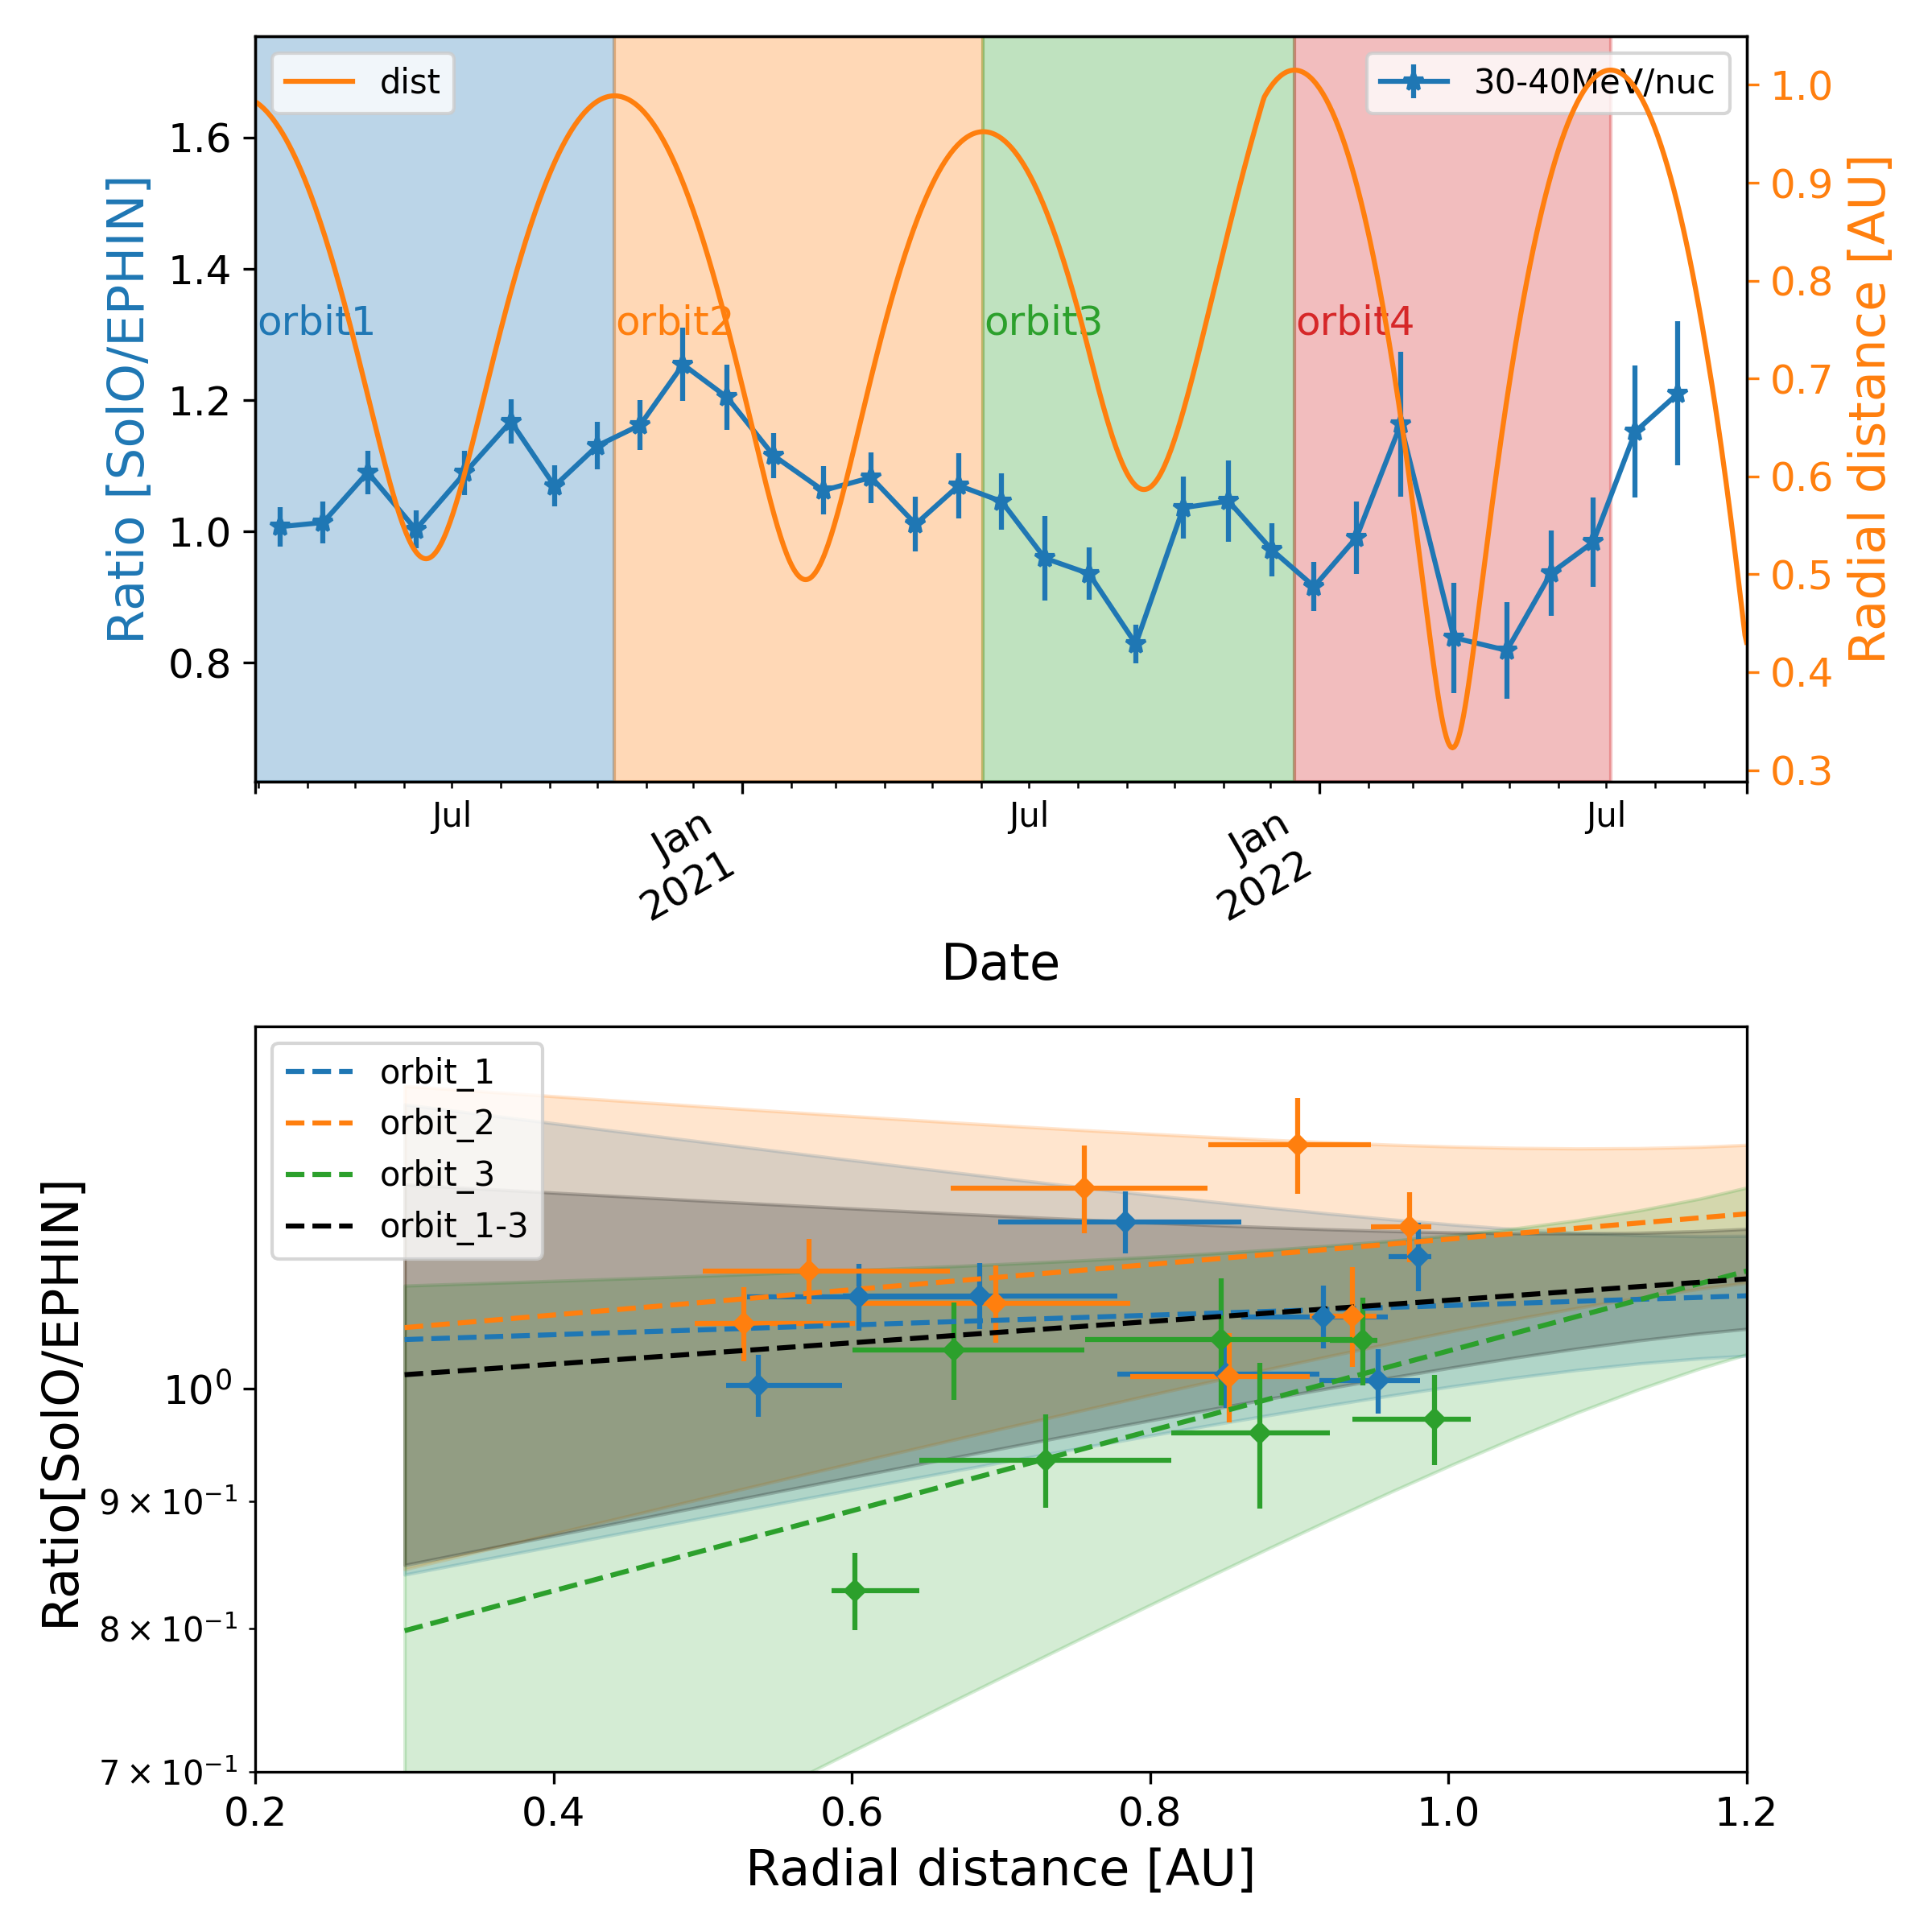
\includegraphics[width =0.48\textwidth, height = 0.3\textheight]{images/ACR/seperate_mask_1-3_newSOHOSEPmask/ratio_time_radialgradient_30-40MeV.png}
    \includegraphics[width =0.48\textwidth, height = 0.3\textheight]{images/ACR/seperate_mask_1-3_newSOHOSEPmask/ratio_time_radialgradient_40-50MeV.png}
    \caption[Ratio of helium intensity between \ac{HET} and \ac{EPHIN} and the radial grdient]{Row 1 and 3: The ratio of helium intensity between \ac{HET} and \ac{EPHIN} in different energy channel changes over times. Row 2 and 4: Ratio vs the radial gradient and the log-linear fitting to the scattering data points for the first three orbit.} 
    \label{fig:ratio_radialgradient}
\end{figure}


\begin{table}[!htb]
    \centering
    \begin{tabular}{|c|c|c|c|c|c|}
        \hline
    Orbit   & 1                 & 2              & 3               & 4  & ave(1-3)\\
    Energy (MeV/nuc)  &         &                &                 &    &\\  
    \hline
    10 - 20 &  0.27 $\pm$ 0.09 & 0.38 $\pm$ 0.14 & 0.21 $\pm$ 0.19 & -0.25 $\pm$ 0.22 & 0.28$\pm$ 0.08\\
    \hline
    20 - 30 &  0.19 $\pm$ 0.09 & 0.28 $\pm$ 0.20 & 0.11 $\pm$ 0.15 & 0.33 $\pm$ 0.16 & 0.19$\pm$ 0.08\\
    \hline
    30 - 40 &  0.05 $\pm$ 0.14 & 0.12 $\pm$ 0.14 & 0.37 $\pm$ 0.21 & 0.08 $\pm$ 0.21 & 0.10$\pm$ 0.11\\
    \hline
    40 - 50 &  0.05 $\pm$ 0.09 & 0.27 $\pm$ 0.21 & 0.58 $\pm$ 0.19 & 0.20 $\pm$ 0.18 & 0.21$\pm$ 0.11\\
    \hline
    \end{tabular}
    \caption[Table of helium radial gradient]{Radial gradient of helium in different energy channels at different orbit between 2020 and 2022.}
    \label{Tab:radialgradient_1}
\end{table}
\subsection*{Radial gradient of helium VS energy}

Fig.~\ref{fig:comparison_SOLO_PSP} displays the dependency of radial gradient on the energy of \ac{ACR} helium. Radial gradients are averaged over the first three orbits and shown as black diamonds, despite of the large uncertainties. Except 30 - 40 MeV/nuc whose average gradient is lower, radial gradients of helium in the remaining energy channels are consistent with each other with uncertainties. For example, we report radial gradients of 0.28$\pm$ 0.08 \%/au, 0.19$\pm$ 0.08 \%/au, and 0.21$\pm$ 0.11 \%/au for helium energies of 10 - 20 MeV/nuc, 30 - 40 MeV/nuc and 40 - 50 MeV/nuc respectviely. Such gradients are also consistent with the \ac{PSP} results within the uncertainties,
To compared with \ac{PSP} results from \citet{Rankin2021ApJ}, we replot helium radial gradients as the blue circles at the similar energy range. \ac{PSP} measurements are from 2018 to 2019, earlier than \ac{SolO}. The averaged radial gradient of helium in the energy range of 4 - 45 MeVn/nuc is about 25$\pm$5 \%/au. 
Besides, the transport model predictions of radial gradient at different energy and different radial distances are plotted as the dashed lines. Data of those lines are from \citet{Rankin2021ApJ,Strauss2010JGRA}.




\begin{figure}[!htb]
    \centering
    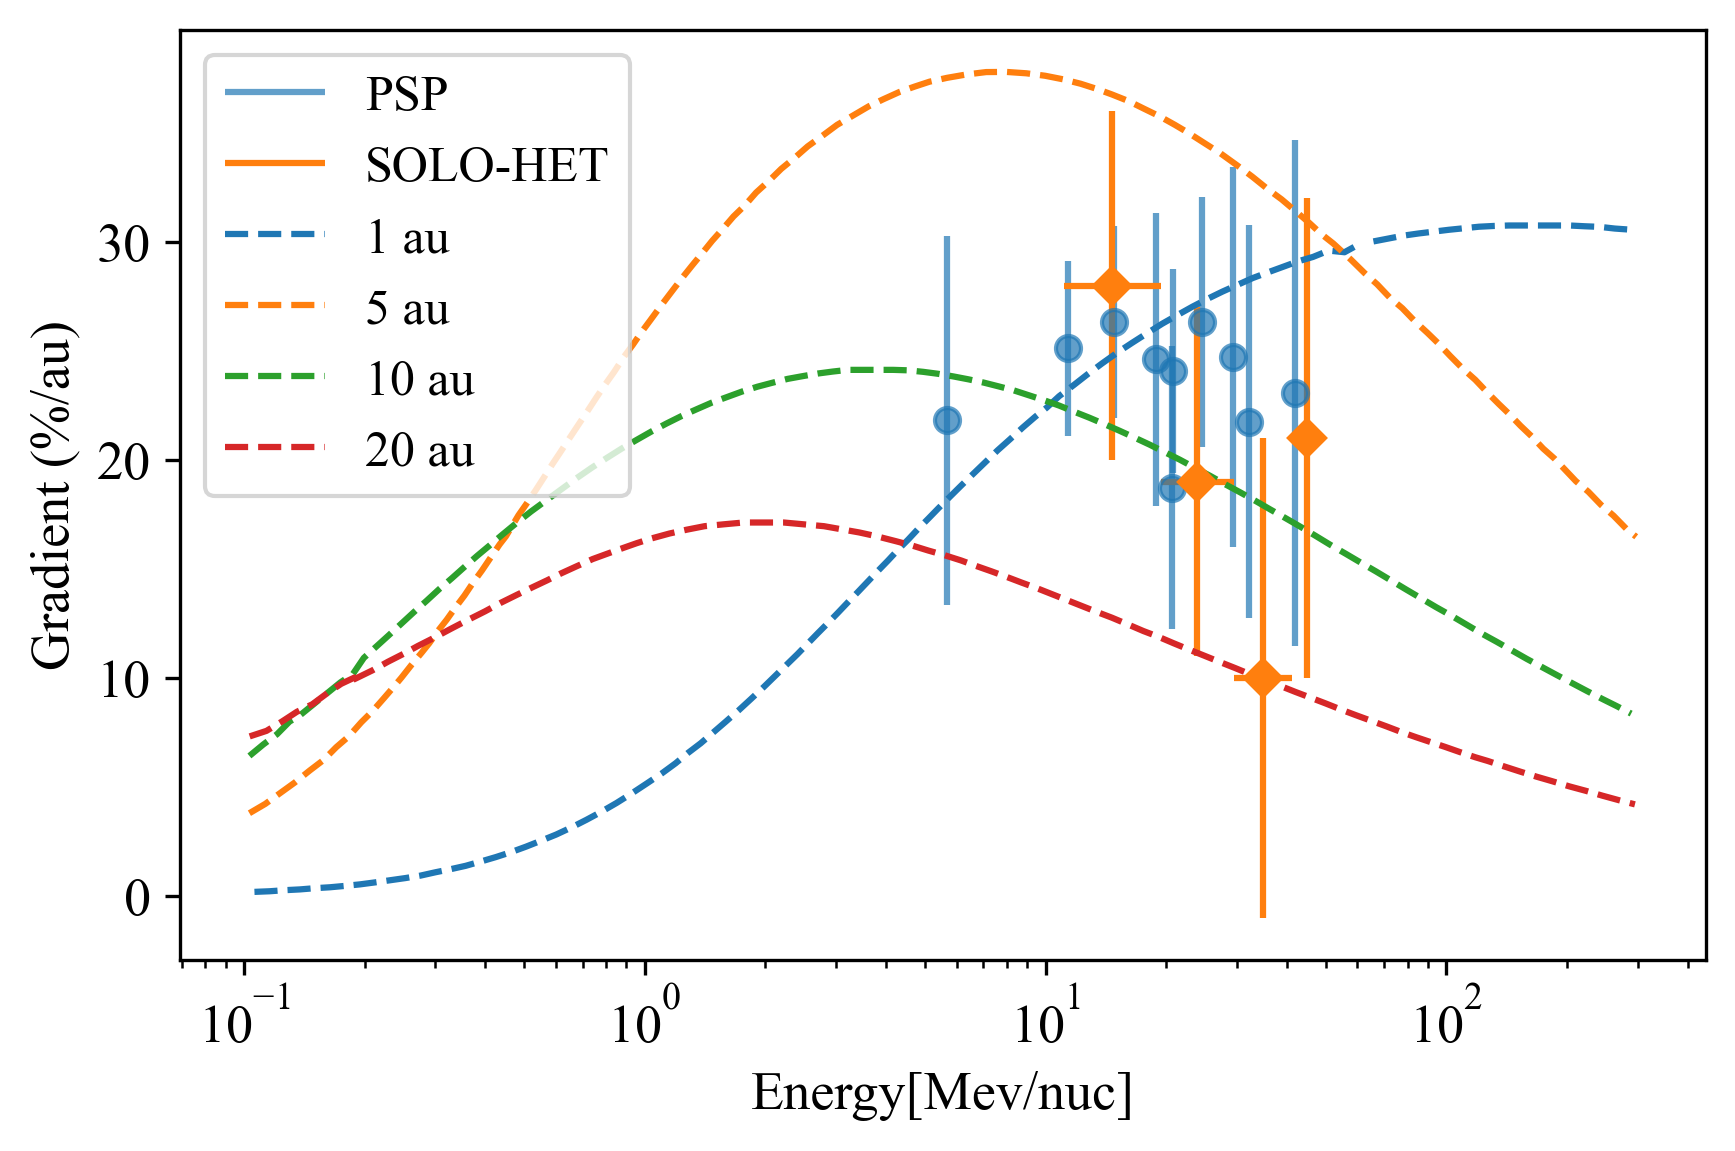
\includegraphics{images/ACR/Energydependent_normal_mask20230612.png}
    \caption[Energy dependency of helium radial gradient]{The radial gradient of helium measured on the ecliptic plane at different energies. The values from \ac{HET} are given as orange diamonds with corresponding error bars. The multiple blue circles in the figure represent the gradient obatained from \ac{PSP} \citep{Rankin2021ApJ}.}
    \label{fig:comparison_SOLO_PSP}
\end{figure}

%  \TODO{New simulation and ask help from some one in Kiel, not now}.


\subsection*{The time variation of the radial gradient}

We also present the time variation of the helium radial gradients for different energy ranges from 10 - 50 MeV in Fig.~\ref{fig:radialgradient_time_variation}. The behaviors exhibited by the different energy channels are distinct, and the radial gradients show significant variations from 2020 to 2022, probablely due to increased solar activity. Several intriguing features are observed in the time variation of the radial gradients, which are unexpected and hard to explain.

It is evident that the peaks of radial gradients occur at different times for each energy channel. The highest radial gradient for the 10 - 20 Mev/nuc helium channel appears during the second orbit, while for the 30 - 50 Mev/nuc channels, the peaked gradients are observed in the subsequent orbit.

Furthermore, the sign of the radial gradient for 10 - 20 MeV/nuc range change from positive to negative during the forth orbit in 2022. This change could potentially be attributed to the larger uncertainties introduced by \acp{SEP}. We removed too much data from \ac{EPHIN} measurements and the few days measurement could not represent the whole carrington rotation, causing that the carrington averaged \ac{EPHIN} flux exhibite more fluctuations compared to the previous periods. The other possible explanation of such a sign change is due to the complicated magnetic field strutures, which changed as solar activities. For instance the radial component near the Sun were overwhelmed by the transverse magnetic fluctuations \citep{Rankin2022ApJ}, causing a completely different tranport environment in the beginning phase of the solar cyle compared to that during the solar minimum.
%From the averaged intensity we could find that the averaged helium flux from \ac{EPHIN} changed drastically between the consecutive carrington rotation. Unlike the similar change in the previous orbit, such change is due to the 
Additionally, during the first two orbit when we were still in the solar minimum phase, the gradient of the 30 - 50 MeV/nuc channel is consistent with zero within the uncertainties and is significantly smaller than the lower energy channels. 

A
\begin{figure}[!htb]
    \centering
    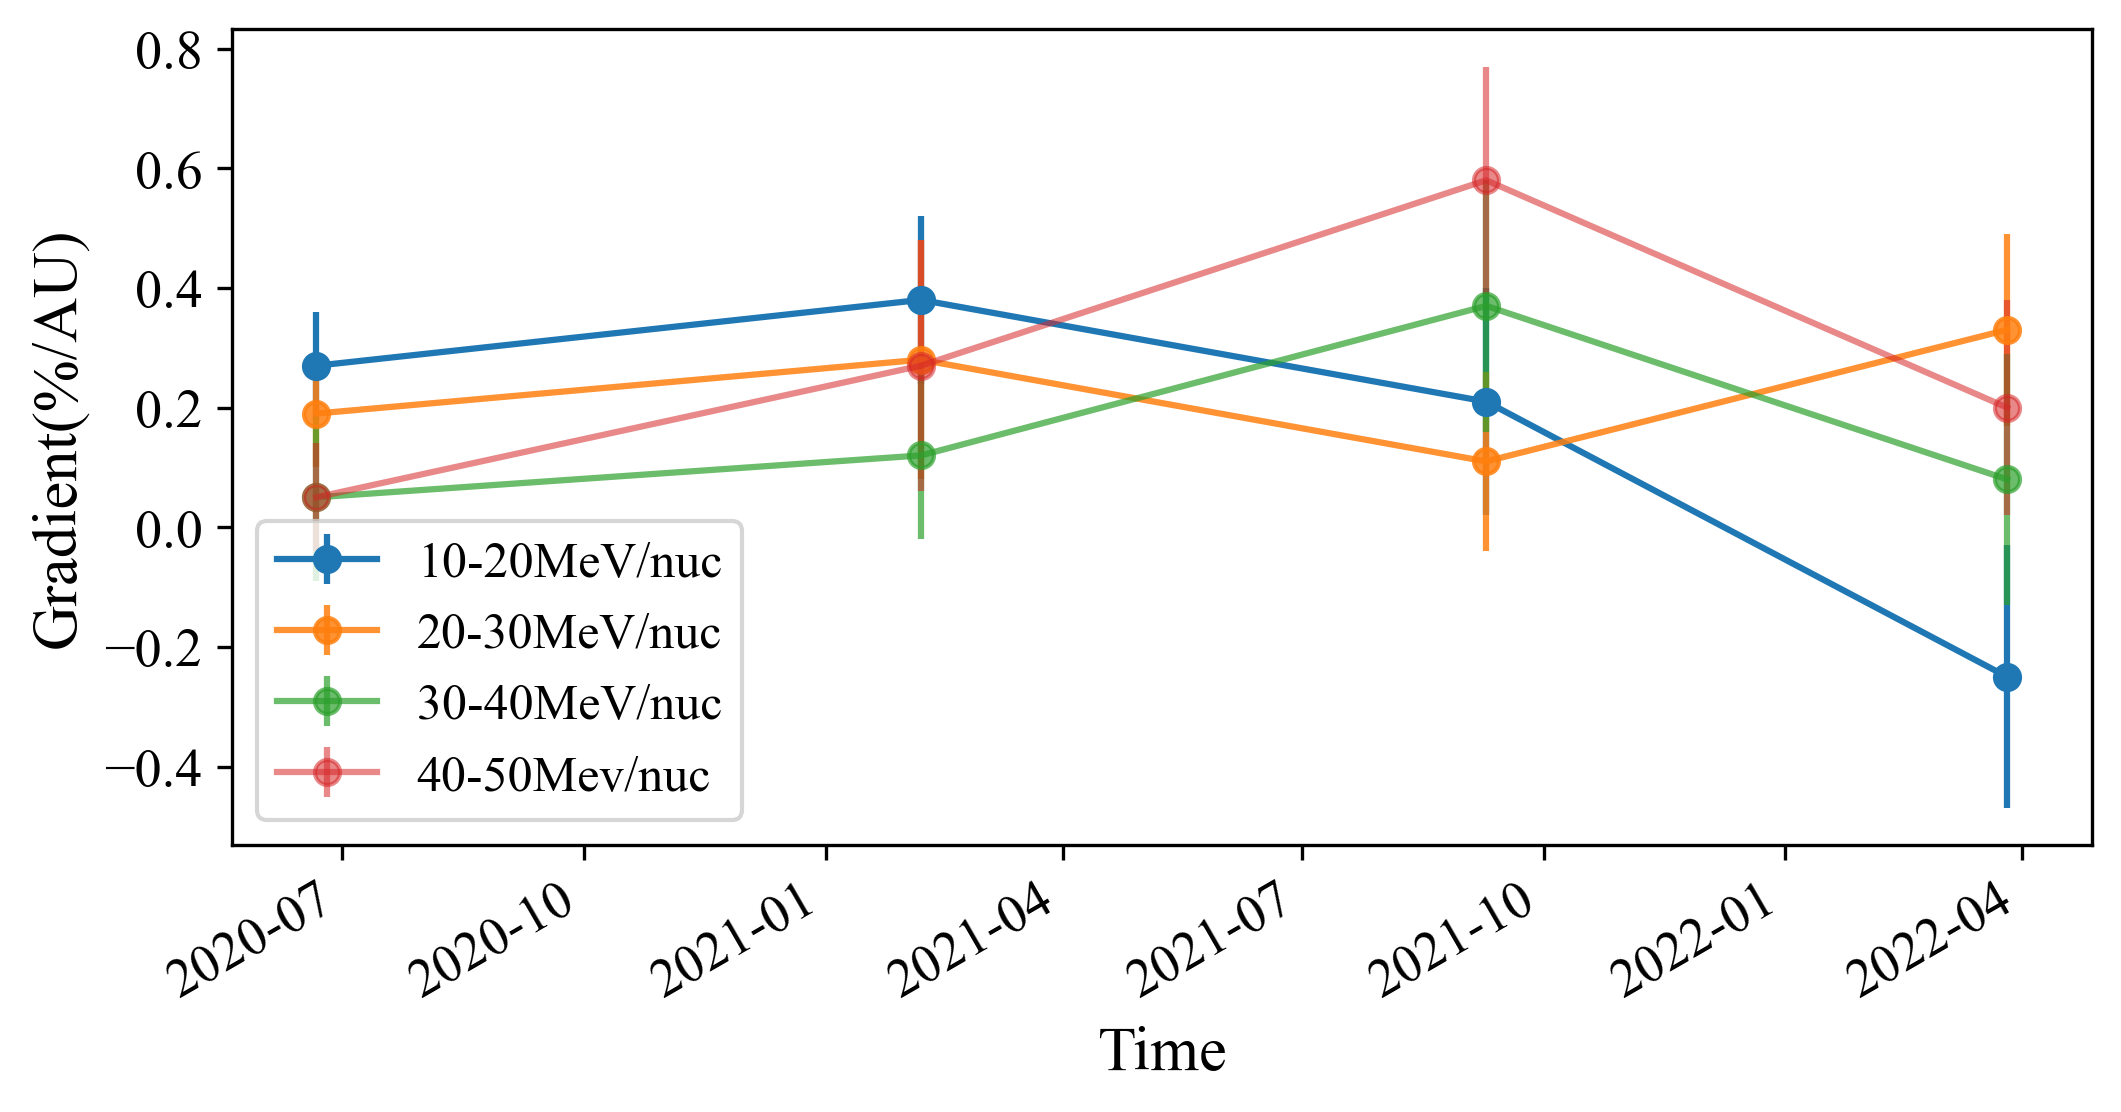
\includegraphics[width = \textwidth, height = 0.3\textheight]{images/ACR/timevariation_normalmask_gradient.png}
    \caption[The time variation of the \ac{ACR} helium radial gradient]{The time variation of the \ac{ACR} helium radial gradient from 2020 to 2022. }
    \label{fig:radialgradient_time_variation}
\end{figure}



\section{ Summary and discussion}

We presented the \ac{ACR} helium in the energy range of 10 - 50MeV/nuc, measured by \ac{SolO}/\ac{HET} between Feb 2020 and Sep 2022. During this periods, the first half was still the solar activity minimum 24/25 characterized by minimal solar activities, while the second half witnessed an increasing number of \acp{SEP}.
Comparisons between the helium spectra obtained by \ac{HET}, \ac{EPHIN} and \ac{ACE}/\ac{ACESIS} show good agreement. Furthermore, \ac{SolO} and \ac{ACE} exhibit consistent measurements for Carbon, Oxygen and Nitrogen as well.

By utilizing the \ac{EPHIN} measurement as the baseline, we derived the radial gradient of \ac{ACR} helium in the inner heliosphere. We removed the effect of long-term solar modulation by divided the intensity of \ac{EPHIN} from \ac{HET}, interference by \acp{SEP}, and the potential short-term variations due to \acp{CIR}.
We reported the radial gradient of 0.28$\pm$ 0.08 \%/au, 0.19$\pm$ 0.08 \%/au, and 0.21$\pm$ 0.11 \%/au for helium energies of 10 - 20 MeV/nuc, 30 - 40 MeV/nuc and 40 - 50 MeV/nuc respectviely. 
These results are consitent with gradients obtained by \ac{PSP} and the prediction of the transport model. Currently those results are very preliminary and more discussions are needed to improve the results.

From the analysis above, we can find how challenging it is to derive the radial gradient of \ac{ACR} helium. In addition to intensity decrease caused by the long-term solar modulation, the more troubled are the remanent \acp{SEP} that could not be recognized from the time series of the proton flux from \ac{EPHIN} and the L2 trigger rate of \ac{HET}. Here we utilize two extra methods over the \ac{SEP} removed intensities of helium to derive a cleaner \ac{ACR} measurements.

In the first method we further removed the data points of high intensity tails during one carrington rotation, in practice we choose the threshold for the highest 5 \% of particles. This method is under the assumption that the highest intensity particle might be from \acp{SEP}. As a result, the radial gradients with extra mask are consitent with the gradients we obtained above. We derive the gradients of 0.27 $\pm$ 0.07 , 0.16 $\pm$ 0.08,0.21$\pm$ 0.11 for helium energies of 10 - 20 MeV/nuc, 20 - 30 MeV/nuc and 40 - 50 MeV/nuc respectviely. 

The second method is based on the assumption that the \ac{ACR} background are rarely changed during certain period, for instance one day. Due to the high time resolution and limited \ac{FOV} of \ac{HET} data products, count rates of helium measurements are discrete values and most of time are zeros. If we assume the background is constant and equal to the mean value,such measurements should follow a Poisson distribution with the $\lambda$ equal to the mean values. When the background is changed, no matter increase or decrease, the Poisson distribution will be changed as well. 
What we did is first calculate the mean value during one day and check how likely the measurements follow the Poisson distribution with the mean value as the $\lambda$.
By doing so, we obtain the same table as the one in Table \ref{Tab:radialgradient_1}, presenting the new results.
The averaged gradients of the first three orbits are 0.34 $\pm$ 0.08 , 0.22 $\pm$ 0.10, 0.19$\pm$ 0.11 for helium energies of 10 - 20 MeV/nuc, 20 - 30 MeV/nuc and 40 - 50 MeV/nuc respectviely. We utilize the Poisson distribution to remove the data points that are not consistent with the background. The results are shown in Fig.~\ref{fig:radialgradient_time_variation}. The gradients are 0.34 $\pm$ 0.08 , 0.19 $\pm$ 0.08,0.21$\pm$ 0.11 for helium energies of 10 - 20 MeV/nuc, 30 - 40 MeV/nuc and 40 - 50 MeV/nuc respectviely.

We also check the result from the other methods including using daily values, using the median flux rather than mean flux represent the flux of center carrrington rotation, both of them give the consistent or the ower radial gradients.

\begin{table}[!htb]
    \centering

    \begin{tabular}{|c|c|c|c|c|c|}
    \hline
    Orbit   & 1                 & 2              & 3               & 4  & ave(1-3)\\
    Energy (MeV/nuc)  &         &                &                 &    &        \\  
    \hline
    10 - 20 &  0.43 $\pm$ 0.10 & 0.21 $\pm$ 0.18 & 0.41 $\pm$ 0.13 & 0.40 $\pm$ 0.49  & 0.34 $\pm$ 0.08\\
    \hline
    20 - 30 &  0.34 $\pm$ 0.13 & 0.23 $\pm$ 0.19 & -0.09 $\pm$ 0.13 & -0.16 $\pm$ 0.28  & 0.22 $\pm$ 0.10\\
    \hline
    30 - 40 &  0.08 $\pm$ 0.15 & 0.19 $\pm$ 0.14 & 0.41 $\pm$ 0.22 & 0.10 $\pm$ 0.20 & 0.13 $\pm$ 0.12\\
    \hline
    40 - 50 &  0.15 $\pm$ 0.04 & 0.15 $\pm$ 0.24 & 0.55 $\pm$ 0.32 & 0.65 $\pm$ 0.33 & 0.19 $\pm$ 0.11\\
    \hline
    \end{tabular}
    \caption[Table of helium radial gradient with extra mask]{The same table as Tab.~\ref{Tab:radiagradient_1} with extra mask to remove the potential short term variation. }
    \label{Tab:radialgradient_2}
\end{table}

Current we just present the result of our analysis for the radial gradient without considering the potential explaination of those features. 
%No matter how, those are the 

% The higher the energy , the deep the particle can penetrate into the heliosphere.

% The higher the solar modulation, the larger the radial gradient.

% General picture: the large the solar modulation, the strong the magnetic field, the large the radial gradient.



% The weak solar magnetic field could not effectively affect the transport of the high energy particles, or at least smaller compared to the lower energy particles.





%\input{chapters/pub04_xu2022}
